\documentclass[11pt]{book}
\usepackage[a4paper, hmargin={4cm, 4cm}]{geometry}
\usepackage{eso-pic} % \AddToShipoutPicture
\usepackage{graphicx} % \includegraphics
\usepackage{minted}
\usepackage{listings}                 % Source code printer for LaTeX
\usepackage{caption}
\usepackage{parcolumns}
\usepackage{fancyhdr}
\usepackage{titlesec}
\usepackage{multirow}
\usepackage{biblatex}
\usepackage{appendix}
\usepackage{tocbibind}
\usepackage{hyperref}
\hypersetup{
    colorlinks,
    citecolor=black,
    filecolor=black,
    linkcolor=black,
    urlcolor=black
}
% Here is where you add your own .bib file
\addbibresource{sources.bib}

\pagestyle{fancy}
\fancyhf{}
\fancyhead[RO, LE]{\thepage}
\fancyhead[LO]{\textsl{\leftmark}}
\fancyhead[RE]{\textsl{\rightmark}}

\renewcommand{\sectionmark}[1]{%
\markright{\thesection \ #1}{}}

\renewcommand{\chaptermark}[1]{%
\markboth{\thechapter \ #1}{}}

\titleformat{\chapter}[display]
  {\normalsize \huge  \color{black}}%
  {\flushleft\normalsize %
   \MakeUppercase{\fontfamily{}\fontsize{24}{24}\selectfont\chaptertitlename}\hspace{2ex}%
   {\fontfamily{}\fontsize{40}{40}\selectfont\thechapter}}%
  {10 pt}%
  {\hrule\vspace{10pt}\raggedleft\bfseries\huge}%


%% Change `ku-farve` to `nat-farve` to use SCIENCE's old colors or
%% `natbio-farve` to use SCIENCE's new colors and logo.
\def \ColourPDF {include/natbio-farve}

%% Change `ku-en` to `nat-en` to use the `Faculty of Science` header
\def \TitlePDF   {include/nat-en}  % University of Copenhagen

\title{
  \vspace{3cm}
  \Huge{A WebAssembly Backend for Futhark} \\
  \Large{Msc Thesis}
}

\author{
  \Large{Philip Lassen}
  \\ \texttt{philiplassen@gmail.com} \\
}

\date{
    \today
}

\usepackage{afterpage}

\newcommand\blankpage{%
    \null
    \thispagestyle{empty}%
    \addtocounter{page}{-1}%
    \newpage}

\newenvironment{longlisting}{\captionsetup{type=listing}}{}

\newcommand{\textBf}[1]{\textbf{#1}}

\AtBeginEnvironment{longlisting}{%
  \renewcommand{\fcolorbox}[4][]{#4}}

\begin{document}


\AddToShipoutPicture*{\put(0,0){\includegraphics*[viewport=0 0 700 600]{\ColourPDF}}}
\AddToShipoutPicture*{\put(0,602){\includegraphics*[viewport=0 600 700 1600]{\ColourPDF}}}

\AddToShipoutPicture*{\put(0,0){\includegraphics*{\TitlePDF}}}

\clearpage\maketitle
\thispagestyle{empty}
\setcounter{page}{0}
\pagenumbering{roman}
\afterpage{\blankpage}


\chapter*{Abstract}
\addcontentsline{toc}{chapter}{Abstract}

Futhark is a high-performance purely functional data-parallel array programming language targeting parallel compute hardware. Futhark has backends for several  compute architectures  and this thesis adds browsers by targeting WebAssembly and threaded WebAssembly. These are browser technologies which map better to the underlying hardware of devices, including multicore CPUs. 

A JavaScript API is developed for easily calling compiled Futhark Web\-Assembly libraries in the browser. 
The implementation and generated Web\-Assembly code is benchmarked for both browsers and Node.js, against the Futhark sequential C and multicore C backends. The sequential Web\-Assembly performs close to sequential C speeds. The parallel execution of threaded Web\-Assembly speeds up some example programs by a factor equal to the number of physical CPU cores.




%A large percentage of today's software is run in the browser, and the underlying hardware of the laptops and mobile phones that run these browser have increasingly parallel compute with GPU's and multicore CPU's. As such there is heavy development of standardized cross browser Web API's to harness these parallel architectures. One of these technologies is threaded WebAssembly. This thesis develops WebAssembly and threaded WebAssembly backends for the Futhark programming language, leveraging both parallel computing and browsers as a target architecture.  


\tableofcontents


\csname @openrightfalse\endcsname
\chapter{Introduction}
\setcounter{page}{1}
\pagenumbering{arabic}
%\section{FIRST ATTEMPT}

%Futhark is a high-performance purely functional data-parallel array programming language targeting parallel compute hardware.
 
%The last two decades have seen the proliferation of consumer devices---laptops, tablets, phones---with parallel computing capabilities with GPUs and multicore CPUs. This is an interesting application space for Futhark.

%A large fraction of the software that runs on these devices runs in the browser. This presents an avenue for executing Futhark on consumer devices if the Futhark compiler can generate code that can run in browsers.

%The WebAssembly browser technology has emerged as a particularly effective compilation target that runs efficiently in the browser.
%Furthermore, WebAssembly has an experimental multithreaded extension called threaded WebAssembly that supports parallel execution on multicore CPUs.

%This thesis develops backends to compile Futhark to WebAssembly and threaded WebAssembly for efficient, parallel execution in web browsers on multicore CPUs, together with a convenient and efficient JavaScript API for Futhark interoperation with browser applications. 

%In this way this thesis contributes towards extending high level and high performance parallel programming to modern consumer devices.




%This thesis is a contribution towards extending high level and high performance parallel programming to modern consumer devices by compiling the functional data-parallel programming language Futhark to WebAssembly and threaded WebAssembly for efficient execution in web browsers on multicore CPUs.

%\section{SECOND ATTEMPT}

%As such there is heavy development of standardized browser APIs to harness these parallel architectures more efficiently than JavaScript. One of the technologies that is getting traction and adoption is WebAssembly which offers near-native single threaded execution speeds in browsers. It is supported by all modern browsers and is the target of compilers for many major programming languages. WebAssembly has experimental support for multithreaded execution with the parallel extension called threaded WebAssembly. It has working compiler and browser support.

The last two decades have seen a proliferation  of consumer devices---laptops, tablets, phones---with parallel computing capabilities with GPUs and multicore CPUs. A large portion of the software running on these devices runs in the browser. 

%, with JavaScript being the standard.

%Emerging technologies are improving how programmers can utilize devices' parallel computing capabilities in the browser.


%Emerging technologies are augmenting standard JavaScript to provide programming tools to utilize devices' parallel computing capabilities in the browser.

%However, the programming tools to utilize devices' parallel computing capabilities in the browser are only just emerging.



%JavaScript is the standard way to 
For decades, JavaScript has been the standard tool for programming in the browser.
JavaScript is ubiquitous but it suffers from inefficient execution. Moreover, there is an increasing interest in compiling other programming languages to run in the browser and JavaScript is not optimal as a compilation target in terms of code size and execution speed. Attempts to solve these issues have led to the development of first asm.js and then WebAssembly, which acts as a kind of assembly language for the browser. WebAssembly is compact and executes at near native speeds and is now supported as a compilation target for many major programming languages, including C, C++, and Rust.
However, WebAssembly is single threaded and doesn't utilize parallel computing capabilites of the underlying hardware.

Development into utilizing parallelism is ongoing with efforts being made both in the context of GPUs and multicore CPUs. One is WebGPU, a proposed web standard and JavaScript API  for calling GPUs in the browser. Another is threaded WebAssembly, an experimental extension to WebAssembly that supports parallel execution on multicore CPUs using Web Workers and provides an interesting compilation target for parallel programming languages to run in the browser.

%It should be noted that WebAssembly is not intended to be used by developers, rather as a compilation target for higher level languages.

Futhark is a high-performance purely functional data-parallel array programming language targeting parallel compute hardware, primarily GPUs. More recently, the Futhark compiler has gained an additional backend targeting multicore CPUs. 

%As a high level programming language, Futhark hides the intricacies of implementing and handling the threads, which would need to be explicitly addressed in a lower level language like C. 

% Parallel is hard 
% Futhark makes easy
% Compiling to browser allows you to compile futhark to any device

%The emerging support for parallel execution in the browser provides an avenue to extend the types of devices that can run futhark code.

This thesis develops backends for compiling Futhark to WebAssembly and threaded WebAssembly for efficient, parallel execution in web browsers, together with a convenient and efficient JavaScript API for Futhark interoperation with browser applications. In this way this thesis contributes towards extending high level and high performance parallel programming to modern consumer devices.

\subsubsection*{Objectives}
The objectives of this thesis are to:
\begin{itemize}


\item Survey technologies for high performance and parallel programming in the browser.

\item Design an API for interoperation between Futhark and browser applications.




\item Implement Futhark backends that generate libraries that run efficiently and in parallel in browsers.

\item Evaluate the performance of these backends. 

\end{itemize}

%The last two decades have seen the proliferation of devices---laptops, tablets, phones---with parallel computing capabilities with GPUs and multicore CPUs.
%A large fraction of today's software runs in the browser.

%{\color{red} TODO}: discuss the challenge of programming browsers to take advantage of the hw

%{\color{red} TODO}: mention the ubiquity and inefficiency of JS

%TODD: mention that WebAssembly is low level, not meant for coding by hand, and therefore a higher level PL is required

%{\color{red} TODO}: argue why Futhark is an interesting source language

%GOALS

%The goal of this thesis is to extend high level and high performance parallel programming to modern consumer devices. (TODO...)

%by compiling the functional data-parallel programming language Futhark to WebAssembly and threaded WebAssembly for efficient execution in web browsers on multicore CPUs.

%This thesis is a contribution towards extending high level and high performance parallel programming to modern consumer devices by compiling the functional data-parallel programming language Futhark to WebAssembly and threaded WebAssembly for efficient execution in web browsers on multicore CPUs.



%A large percentage of today's software is run in the browser, and the underlying hardware of the laptops and mobile phones that run these browser have increasingly parallel compute with GPU's and multicore CPU's. As such there is heavy development of standardized cross browser Web API's to harness these parallel architectures. One of these technologies is threaded WebAssembly. %This thesis develops WebAssembly and threaded WebAssembly backends for the Futhark programming language, leveraging both parallel computing and browsers as a target architecture.




\subsubsection*{Thesis Structure}
This thesis is organized with the following structure:

\begin{itemize}

\item Chapter 2, Background:
    Overview of the related work that this thesis builds on.

\item Chapter 3, WebAssembly:
    Explanation and analysis of WebAssembly as a programming language and as a target language for the browser. 

\item Chapter 4, API Design:
    We develop an API for calling Futhark Web\-Assembly libraries from JavaScript. 

\item Chapter 5, WebAssembly Backend:
    Description of the implementation of the WebAssembly backend. As well as a overview of the performance bench-marked against the native C backend.
    
\item Chapter 6, Parallel Execution in the Browser:
    Analysis of the facilities and paradigms for parallel programming in the browser through JavaScript and WebAssembly. 
    
\item Chapter 7, WebAssembly Multicore Backend:
    Description of the implementation of the multicore WebAssembly backend. As well as an overview of the performance benchmarked against the native multicore C, and WebAssembly backend developed in Chapter 5.
    
\item Chapter 8, Conclusion:
    Summary of the implementations and performance of the backends and API developed. As well as a brief discussion of future developments for Futhark targeting parallel compute in the browser.
    
\end{itemize}

\chapter{Background}

This chapter describes relevant background for the work in this thesis, namely browser programming facilities and the Futhark programming language.




\section{Programming Languages in the Browser}

%\section{Futhark}


%\section{Browsers}

%The first web browsers started as Graphical User Interfaces for rendering static web pages. Web Browsers have evolved to keep up with the high paced innovation in web technologies and with modern day browsers having strong similarities with full blown operating systems. 


%\subsection{JavaScript}

%JavaScript for a long period of time was the only supported programming language for the browser. As such it became one of the largest programming languages in the world. With browsers being one of the most ubiquitous coding platforms, programmers were restricted to JavaScript for any functionality in their websites that run client side. As a result many languages added backends to target JavaScript to that programmers could write code in their respective languages and generate JavaScript that would run in the browser. The problem is that JavaScript is not a particularly good target language, as it was not designed with this use case in mind. 

%http://www.observationalhazard.com/2018/06/history-of-web-programming.html
% ^ This is about the programming languages in the web in the early days vbscript and java applets

In the early days of web browsers, web pages would render differently across browsers as web APIs were not standardized. Different browsers supported different programming languages, e.g. Java applets and VBScript, creating headaches for programmers who wanted their websites to render identically across browsers. The first popular language for the browser was JavaScript, but the implementations across browsers differed. Eventually the big vendors converged on JavaScript releasing a standardized version called ECMAScript. 

Huge investments have been made to increase the execution speed of JavaScript in the browser. 
All the major browser vendors have optimized the performance of their JavaScript engines, in particular V8 in Chrome and SpyderMonkey in Mozilla. Many approaches have been taken to make JavaScript faster but they have all been fundamentally limited by the language design. 

%\subsection{ASM.js}

One of the approaches taken by the browser vendors was to define a subset of the language asm.js and a convention for type hints, which were designed for efficient execution by leveraging types and compiler tricks to allow ahead-of-time compilation. It was intended as a target language for compilation of statically typed programming languages. Emscripten \cite{emcc} was developed to be a C/C++ to asm.js compiler. 

Google also introduced Google Native Client (NaCl) \cite{nacl} as a way to bridge the speed gap between running code in the browser, and natively. NaCl is a sandbox for running compiled C and C++ code in the browser efficiently and securely, independent of the user’s operating system \cite{nacl}. However it struggled to gain adoption due to its lack of portability as it was only supported by Chromium based browsers. 


%\subsection{WebAssembly}
The major browser vendors collaboratively designed WebAssembly (Wasm) \cite{wasm_og} to more comprehensively address the limitations of JavaScript as a target language for the web. It is a portable low level byte code, designed for compact representation, efficient compilation, and near native execution speeds. Web\-Assembly is gaining adoption and has been used for a variety of applications especially as a target for compilation from C, C++ and Rust. 

Google Earth \cite{google-earth-history} is an example of a major application that is adopting WebAssembly. Google Earth renders a 3D representation of Earth based primarily on satellite imagery. It started out as a desktop application, but in 2013 was ported to the web. It originally only ran in Chrome, as it was built on NaCl. The developers tried to build it with asm.js, but found the binary sizes of compiling over a million lines of code with Emscripten to be infeasibly large. However with the creation of WebAssembly they were able to make a high performance cross browser implementation of Google Earth due to the speed and small binary sizes of WebAssembly \cite{google-earth}.

Another example is TensorFlow \cite{tensorflow}, an open source machine learning library, originally written in C++. Due to the large eco-system of JavaScript developers and its ability to run on the browser, the developers introduced TensorFlow.js \cite{tensorflowjs}. They have multiple backends including a WebAssembly backend, which is 10-30x faster than their plain JavaScript backend \cite{tf-speed}. What is interesting about TensorFlow.js is that it shows how WebAssembly can be used to create high performance libraries that can be called from the web.


%\section{LLVM}

One of the technologies that has greatly helped the adoption of WebAssembly as a target language is the LLVM \cite{llvm} compiler tool chain. Writing a full compiler from scratch that supports multiple targets is a huge undertaking. In order to have high performance backends for different target architectures such x86 and ARM requires knowledge of many of the low level details of each respective target. An alternative approach is for the compiler frontend of the source language to take the source code and translate it to the LLVM internal representation (IR). The LLVM compiler tool-chain can then generate high performance code on all the most common computer architectures. Many of the biggest languages are currently built with or have compiler implementations using LLVM.
LLVM compiles from its IR to WebAssembly and therefore languages that generate LLVM IR have an easy path to WebAssembly code generation. 
Emscripten uses LLVM and can generate WebAssembly in addition to asm.js. It is a widely used compiler for generating WebAssembly.

\section{Parallel Programming in the Browser}
While WebAssembly has progressed the state of the art of single threaded computation speed in browsers another avenue for execution speed is parallelism. Browsers have facilities for parallel programming. Javascript supports two different paradigms with web workers. Message passing enables parallel programming without shared  memory. SharedArrayBuffer and atomics enable shared memory multithreading with thread synchronization.  There is a threaded WebAssembly proposal that adds atomic operations to the language, and adds support for SharedArrayBuffers while relying on JavaScript’s web workers to create and join threads. Emscripten can currently compile C with POSIX threads to threaded WebAssembly. The Chrome and Firefox browsers along with Node.js have experimental support for threaded WebAssembly.

%{\color{red} TODO} mention GPU API's for the browser

\section{Futhark}


Futhark \cite{futhark-og} \cite{futhark_phd} is a data parallel programming languages that can generate high performance parallel code for both the CPU and GPU .  Writing GPU code and multicore CPU code is difficult as there are many low level details required to make correct and optimal implementations. Futhark is a high level functional programming language, which aims to do the heavy lifting for the user.



Futhark programs are generally written with Second-Order Array Combinators (SOACs), which are similar to the filter, map, and reduce functions commonly found in many functional programming languages. These functions can be optimized to efficient parallel code. These combinators are  expressive and be combined to encode code complex programs. 
%
%This thesis is not going to explain the Futhark language. Most of the Futhark code snippets scattered throughout the thesis are short and easy to understand without prior familiarity to the language.
%
To see this in action below is a Futhark implementation of matrix multiply:
\begin{verbatim}
let matmul [n][p][m] (xss: [n][p]f64) (yss: [p][m]f64): [n][m]f64 =
    let dotprod xs ys = reduce (+) 0 (map2 (*) xs ys)
    in map (\xs -> map (dotprod xs) (transpose yss)) xss
\end{verbatim}
Here \texttt{dotprod xs ys} computes the dot product of two vectors \texttt{xs} and \texttt{ys} by computing the pairwise products \texttt{zs = map2 (*) xs ys} and then summing the products with \texttt{reduce (+) 0 zs}.
In the last line the innermost \texttt{map} in \texttt{map (dotprod xs) (transpose yss)} computes a row vector of the product matrix and the outermost \texttt{map} generates all the rows.

This serves as an illustration of how a relatively involved operation can be written using SOACs. Not only is the implementation short, it's also fast.

This thesis is not going to explain the Futhark language in further detail. Only very short Futhark functions will be used in examples and do not require deeper understanding of the language.

Currently the futhark compiler has C backends generating Cuda, OpenCL, and sequential C code. Recently a multicore C backend was added that generates parallel code using POSIX threads (pthreads) \cite{multicore}. Futhark also has two Python backends, one sequential and one using PyOpenCL. All the backends can be compiled to libraries, making it possible to call Futhark from C or Python applications. For this this thesis we build off of the sequential C backend and the multicore C backend. 


%The plain C code backend comes in two variants, sequential C and multicore C. The latter is a recent addition and generates parallel code using POSIX threads (pthreads) \cite{multicore}. These backends are important for this thesis. Emscripten compiles sequential C to plain WebAssembly, and C with pthreads to threaded WebAssembly. This allows us to bootstrap these two backends to generate efficient code that can run in the browser. 


%TODO: explain which of the alternatives we chose


\chapter{WebAssembly}
This chapter gives an overview of the design and structure of the WebAssembly programming language. We illustrate the instruction set with two simple hand written WebAssembly modules. We show how functions and memory work, and how to call a module from JavaScript. Most importantly we show how to generate WebAssembly and JavaScript glue code with Emscripten and how to work with Emscripten's JavaScript API.

%This will be driven through an example program, and some performance evaluations and literature review. 



%Its important to note that WebAssembly doesn't aim to be a complete replacement for JavaScript. WebAssembly cannot access the DOM for example. WebAssembly was instead designed to have good interoperation with JavaScript. In practice a developer wanting to get high performance code running in the browser would first write their library in a language such as C or Rust. Then they would compile to WebAssembly, and use JavaScript to call their WebAssembly module in the browser. 




%WebAssembly defines a portable binary format that can be run in the web with high performance. 



\section{WebAssembly Module Structure}

This section describes some of the lower level details of the WebAssembly programming language. They illustrate some of WebAssembly's characteristics but they are not critical for understanding the rest of the thesis.

A WebAssembly file is commonly referred to as a module, and given a \textit{.wasm} file extension. WebAssembly also defines a text format that serves to be a human readable version of the underlying binary format, much in the same way assembly provides a human readable format for machine code. The \texttt{wat2wasm} program from The WebAssembly Binary Toolkit\footnote{https://github.com/WebAssembly/wabt}
compiles the textual format to a binary module.

WebAssembly modules are segmented into sections. The segmentation of these sections is done so that loading a WebAssembly file is as efficient as possible. The sections are structured such that the byte code can be compiled in a single pass, and in parallel. Furthermore the code can be parsed and compiled before the complete WebAssembly file has been downloaded, reducing the instantiation time of a WebAssembly module. 

WebAssembly supports the 4 number types of 32-bit and 64-bit integers, \texttt{i32} and \texttt{i64}, and floats, \texttt{f32} and \texttt{f64}. These don't map cleanly to JavaScript's number types but are useful for supporting number types for languages like C/C++ and Rust, the languages it aims to be a target language for. 

A WebAssembly function has the following structure.
\begin{verbatim}
( func <signature> <locals> <body> )
\end{verbatim}
The signature gives the function name, parameter types, and return types. The locals are the local variables that will be used in the execution of the function, and the body is the actual implementation of the function. A simple WebAssembly example is the add function. 

\begin{verbatim}
(module
  (export "add" (func $add))  
  (func $add (param $a i32) (param $b i32) (result i32)
    local.get $a
    local.get $b
    i32.add
  )
)
\end{verbatim}

The function signature of add specifies the two arguements a and b as \texttt{i32} and specifies the return type result as \texttt{i32}. There are no locals. The function body has three instructions. The instructions \texttt{local.get \$a} and \texttt{local.get \$b} push the two arguments to onto the stack. The instruction \texttt{i32.add} pops the two elements off the stack and pushes their sum. The function returns the number on the stack. 

The body of the function could be replaced with:
\begin{verbatim}
 (i32.add (local.get $a) (local.get $b))
\end{verbatim}
That is, WebAssembly allows the programmer to use a notation where arguments to instructions are passed as parameters instead of manually being placed on the stack.



%{\color{red} TODO} link and ref mdn https://developer.mozilla.org/en-US/docs/WebAssembly/Understanding_the_text_format
\section{Memory}

A notion of memory is needed for writing more complex programs. In a language like C, it is common practice to use pointers to locations in memory, or for writing an array of values. Memory from the perspective of WebAssembly is just an array of bytes that can be read from and written to. WebAssembly has two essential functions for interacting with this array, namely the \texttt{load.i32} and \texttt{store.i32}, for reading and writing to the array of bytes respectively.

As a motivating example, the following C code gives a simple implementation of a place prefix sum. (Again, this example is just for illustration and not needed to understand the rest of the thesis.)

\begin{verbatim}
void prefix_sum(int* arr, int size) {
  for (i = 1; i < size; i++) {
    arr[i] += arr[i-1];
  }
}
\end{verbatim}
The following code is a WebAssembly implementation of in-place prefix sum.
\begin{verbatim}
  1 (module
  2   (import "env" "memory" (memory $memory 1))
  3   (export "prefixSum" (func $prefixSum))
  4   (func $prefixSum (param $size i32)
  5     (local $offs i32)
  6     (local $acc i32)
  7     (local $last i32)
  8     (local.set $offs (i32.const 4))
  9     (local.set $last (i32.mul (local.get $size) (i32.const 4)))
 10     (local.set $acc (i32.load (i32.const 0)))
 11     loop $forloop
 12       (local.set $acc (i32.add (local.get $acc) 
                         (i32.load (local.get $offs))))
 13       (i32.store (local.get $offs) (local.get $acc))
 14       (local.set $offs (i32.add (local.get $offs) (i32.const 4)))
 15       (br_if $forloop (i32.ne (local.get $offs) 
                                  (local.get $last)))
 16     end $forloop
 17   )
 18 )
\end{verbatim}
% {\color{red} TODO} brief description of WebAssembly
% {\color{red} TODO} talk about 64k pages

For the implementation, a local variable accumulator is set to the first value of the array and an offset is set to 0. A loop is then entered, where the element at offset in the array is loaded with \texttt{i32.load} and added to the accumulator, \texttt{\$acc}. The result is stored with \texttt{i32.store}. The offset is increased by 4 bytes, and then compared to the local variable \texttt{\$last}. If it is not equal the loop goes back to the loop on line 12, and repeats.

The most important details of the function implementation for understanding WebAssembly's interaction with memory are the load and store operations, which use byte offsets to address memory. The memory is never explicitly referenced in the function because WebAssembly modules only have one declaration of memory in the memory section, making the array of memory implicit. Memory can either be imported from JavaScript, in which case the memory is created in JavaScript and passed to WebAssembly on instantiation, or, alternatively, the memory can be exported from WebAssembly, in which case the memory is created in WebAssembly on instantiation and can be accessed in JavaScript afterwards. The memory is imported in line 2:
\begin{verbatim}
(import "env" "memory" (memory $memory 1))
\end{verbatim}
The ending, 1, sets the size of the memory heap to be 1 page of memory. For WebAssembly 1 page corresponds to 64 kilobytes. Memory is always set to an integer number of pages.


\section{WebAssembly and JavaScript Interaction}

%WebAssembly defines a small set of instructions, which runtimes can translate to native code quickly. However because of this it is unable to complete many of the basic functions of JavaScript. 

Listing \ref{lst:add.html} shows how to load, instantiate, and call the \textit{add.wasm} module from JavaScript in a web page.
\begin{listing}[h] 
\inputminted[fontsize=\small,baselinestretch=0.5,linenos]{HTML}{code/examples/wasm/add.html}
\caption{Invocation of \textit{add.wasm} in web page}
\label{lst:add.html}    
\end{listing} 


By design a WebAssembly module only interfaces with its environment through function inputs and outputs, and through memory. 
The most clear cut example of this is the lack of access to the DOM. 
WebAssembly does not have direct access to Web APIs. However it can call imported JavaScript functions. This facility allows it to interact with Web APIs. This simple design feature is powerful. It is this feature that enables threaded WebAssembly as it can leverage JavaScript's ability to spawn web workers. This will be discussed in greater detail in Chapter 6. %OBS


%For most practical use cases WebAssembly modules are used as libraries.



\section{Emscripten}
This section describes how to generate WebAssembly and JavaScript glue code with Emscripten and how to work with Emscripten's JavaScript API. This material is critical for understanding the backend implementation in chapter 5. 

As described in chapter 2, the popular
Emscripten toolchain compiles C/C++ to a WebAssembly module. It also generates JavaScript "glue code", a phrase we use with the specific meaning of code that Emscripten generates to encapsulate module instantiation and access through Emscripten's JavaScript API.
Technically the library user can load the WebAssembly module directly as in listing \ref{lst:add.html}. However this is impractical for a couple of reasons. The module is constructed by Emscripten to import a series of system library functions to access files and allocate memory etc. Emscripten's glue code supplies all these at instantiation time and hides this from the library user.



%When compiling C to WebAssembly as a library the Emscripten compiler generates two files. One is a WebAssembly module and the other is JavaScript glue code. This allows web programmers to access all the important elements of WebAssembly from a set of JavaScript functions that the Emscripten runtime defines. This is beneficial for multiple reasons. Firstly working directly with WebAssembly modules is a layer of detail most web developers would like to avoid. Secondly this approach allows a programmer to simply compile their C library and call it from JavaScript. 

%It is impractical to work with WebAssembly as a modules directly. There are many low level details in terms of interacting with memory and instantiating a WebAssembly module that programmers would like to avoid. For this reason Emscripten also generates JavaScript glue code. 

For many use cases, compiling code to a library is desirable. This way a programmer can write source code in C/C++ that contains functions for compute intensive parts of their application. They can then generate WebAssembly modules that can be called from JavaScript, and offload the computation to WebAssembly. 

It is relatively straightforward to call simple C functions from JavaScript when they are compiled with Emscripten. We just need to explicitly export the functions at compile time.

If we have a simple C file \textit{add.c} that contains an add function.
\begin{verbatim}
int add(int a, int b) { return a + b; }
\end{verbatim}
We compile with Emscripten to a library while making sure to export the function.
\begin{verbatim}
emcc add.c -o add.js -s MODULARIZE -s EXPORTED_FUNCTIONS=[_add]
\end{verbatim}
We also use the MODULARIZE flag, to make the WebAssembly Module easier to import. This is helpful because WebAssembly is loaded asynchronously. With the MODULARIZE flag we are able to get the module as a promise. The following code runs in Node.js:
\begin{verbatim}
var load_module = require('./add.js');
load_module().then((instance) => {
  console.log(instance._add(4, 6));
});
\end{verbatim}
The \texttt{load\_module} is a factory function. Once the WebAssembly Module is loaded we run the code in the callback. The actual logic for running the C function is just the one line:
\begin{verbatim}
  console.log(instance._add(4, 6));
\end{verbatim}
The example library can also be loaded as a script in a web page and invoked from JavaScript in the browser. This will be shown later in the Mandelbrot example in Section \ref{sec:mandelbrot}.

Library functions compiled with Emscripten are easy to use when they take integer arguments and have integer return types. However lots of C/C++ works with pointers. Emscripten models that with locations in a single memory region attached to the WebAssembly module. This memory region is called the heap. Emscripten offers multiple views into the heap with a typed array for each primitive element type, namely those supported by JavaScript typed arrays. See Table \ref{table:heapviews}. These typed array all share the same underlying ArrayBuffer memory.

%Note that pointers default to 32-bit signed integers in WebAssembly and are therefore written to and read from memory using the HEAP32 heap view.\footnote{{\color{red} TODO}: wasm64}

\begin{table}[H]
\centering
\begin{tabular}{|l|r|}
\hline
\textBf{Heap view} & \textBf{JavaScript type} \\ \hline
\texttt{HEAP8} & \texttt{Int8Array} \\ \hline
\texttt{HEAP16} & \texttt{Int16Array} \\ \hline
\texttt{HEAP32} & \texttt{Int32Array} \\ \hline
\texttt{HEAP64} & \texttt{BigInt64Array} \\ \hline
\texttt{HEAPU8} & \texttt{Int8Array} \\ \hline
\texttt{HEAPU16} & \texttt{Uint16Array} \\ \hline
\texttt{HEAPU32} & \texttt{Uint32Array} \\ \hline
\texttt{HEAPU64} & \texttt{BigUint64Array} \\ \hline
\texttt{HEAPF32} & \texttt{Float32Array} \\ \hline
\texttt{HEAPF64} & \texttt{Float64Array} \\ \hline
\end{tabular}
\caption{Emscripten's heap views and their JavaScript types}
\label{table:heapviews}
\end{table}

Typed arrays will play an important role in this thesis, both for interacting with the Emscripten heap and for array parameters to compiled Futhark functions. Typed arrays are useful because they represent number arrays compactly and efficiently, and the ability for typed arrays to act as different views of the same underlying ArrayBuffer can be used to avoid memory copies for parameter passing in many cases.

To illustrate how to pass pointer arguments, consider the simple C string function in listing \ref{lst:concat-c} which takes two strings and return their concatenation into allocated memory that the caller must free.

\begin{listing}[h!] 
\inputminted[fontsize=\small,baselinestretch=0.5,linenos]{C}{code/examples/emcc/concat.c}
\caption{C concat function }
\label{lst:concat-c}    
\end{listing} 

To use this function the caller will need to use the malloc and free system library functions, so we export those alongside concat when we compile to a library with Emscripten:
\begin{verbatim}
emcc concat.c -o concat.js -s MODULARIZE \
  -s EXPORTED_FUNCTIONS=[_malloc,_free,_concat]
\end{verbatim}

The Node.js program in listing \ref{lst:hello-world.js} calls concat.
\begin{listing}[H] 
\inputminted[fontsize=\small,baselinestretch=0.5,linenos]{C}{code/examples/emcc/hello-world.js}
\caption{Node.js call to Emscripten compiled concat function }
\label{lst:hello-world.js}    
\end{listing} 

The pointers a and b passed to \texttt{\_concat} are locations in the Emscripten heap, so the caller must first copy the strings to the heap for \texttt{\_concat} to access them. To find a place in the heap to place them, we call \texttt{malloc} twice and then use the \texttt{HEAPU8} heap view to write the strings into the allocated memory.
We zero terminate the a string with:
\begin{verbatim}
instance.HEAPU8[a + alen] = 0;
\end{verbatim}
and write into the first \texttt{alen} bytes through:
\begin{verbatim}
instance.HEAPU8.subarray(a, a + alen)
\end{verbatim}
It is another Uint8Array which is a view into the subarray of the heap that holds the first alen bytes, up to and excluding the terminating zero. 
The returned pointer, \texttt{c}, again points into the heap and we find the heap location of the terminating zero with:
\begin{verbatim}
var cend = instance.HEAPU8.indexOf(0, c);
\end{verbatim}
and then we get a view of the concatenated string with:
\begin{verbatim}
instance.HEAPU8.subarray(c, cend)
\end{verbatim}
Finally, all the allocated strings are freed with calls to \_free.


Emscripten's function and heap API and compiler flags will play important roles in the implementation of the WebAssembly backends for Futhark in chapter 5 and 7.



%\section{WebAssembly outside the browser}

%There are also a number of applications for WebAssembly outside of the browser. The most standard engine for running WebAssembly outside the browser is Node. Node also uses the V8 engine that is present in Chrome, and other browsers to support WebAssembly. As a result it is a high degree of performance parity with WebAssembly that is run in the browser.

%Running Node locally is convenient for rapid prototyping as well as testing. Making tests that run in the browser takes a deal of configuration, and isn't trivial. It is possible to run Chrome, and Firefox as headless browsers for testing purposes, but often it is desirable to test part of WebAssembly functionality


%WebAssembly executes within a sand-boxed stack-based environment, which means that running foreign code can only effect the virtual environment that executes the WebAssembly module. This compounded with its competitive performance to native code makes it an ideal candidate for any applications that need to run foreign code. 

\chapter{API Design}


The WebAssembly backends that we are going to develop will compile Futhark functions to libraries for use in the browser. This section designs a JavaScript API for programs in the browser to call the compiled library functions.


%to call the WebAssembly modules from the browser, an efficient, convenient, and concise JavaScript API was developed and illustrated with examples






%This chapter describes the implementation of an additional Futhark backend that generates WebAssembly and JavaScript code such that Futhark programs can be compiled to libraries that can be run in the browser. The implementation includes an API to invoke the compiled libraries from JavaScript. The implementation is benchmarked in the Chrome browser, and in Node.js and against the C backend.

%Firstly we design the JavaScript API. We take inspiration from the Futhark C and Python APIs. Our design factors in the characteristics and limitations of JavaScript and WebAssembly. The API is illustrated with an example.%OBS



%Secondly we implement the backend. We take outset in the existing futhark Sequential C backend and pass the generated C code to the Emscripten compiler for the final compiler pass. The Emscripten generates a WebAssembly module along with JavaScript glue code. We generate additional JavaScript code to wrap our API around the JavaScript code generated by Emscripten.

%To illustrate the API and backend implementation working in practice we use the WebAssembly backend to efficiently generate graphics for the Mandelbrot set in a webpage.

%Finally we benchmark the Futhark backend to quantify its performance. The benchmarks come from the futhark benchmark suite\footnote{https://github.com/diku-dk/futhark-benchmarks}, which are standardized benchmarks to test the performance of Futhark backends against industry standards. The benchmarks show the WebAssembly, both when run in the Browser and run on Node locally, performs between 12\% to 65\% slower than the generated C running locally. 

%\section{API Motivation}

In order to make Futhark a practical language for writing libraries that can be called in the browser it is important that it has a simple and efficient API. As discussed in chapter 3 code that is compiled to WebAssembly modules typically comes packaged with a JavaScript file. This file contains the library functions that are exposed to the programmer, where internally these functions handle the interaction with WebAssembly. This allows users of the library to be oblivious of the fact that WebAssembly is being used under the hood, much in the same way that some Python developers are oblivious that numpy is running compiled C under the covers.

A successful API for calling Futhark in the browser will have the following properties
\begin{enumerate}
    \item It should be convenient, seamlessly integrating with the most commonly used JavaScript number and array data types.
    \item The API should be efficient both with respect to memory usage and runtime speed.
    \item Finally the API should minimize boiler plate code.
\end{enumerate}

\section{Comparing Futhark APIs}

It is insightful to look at the APIs of other languages so that we can copy the elements of the APIs that are effective and avoid the parts that are cumbersome or inefficient. These decisions are constrained by the limitations and capabilities of the target language, which for us is JavaScript and WebAssembly.

An additional reason why it is important to observe the C API, is that the WebAssembly backend builds off the sequential C backend. For this reason our design choices for the API are limited to how we can wrap the C API function calls behind JavaScript classes and functions.
%% MAYBE Section not CHAPTER BE MINDFUL YOUNG CHILD

The exposition will be example based.
The first example is the minimal program in listing \ref{lst:simp} that takes a 32 bit integer and returns the successor.
\begin{listing}[H]
\begin{minted}{Haskell}
entry increment (a : i32) = a + 1
\end{minted}
\caption{Futhark increment function, \textit{increment.fut}}
\label{lst:simp}
\end{listing}

The second example in listing \ref{lst:scale} works with multidimensional array inputs and outputs as well as a scalar input:
\begin{listing}[H]
\begin{minted}{Haskell}
entry scale (scalar : f32) (matrix : [][]f32) = 
  map (map (scalar *)) matrix
\end{minted}
\caption{Futhark scale function, \textit{scale.fut}}
\label{lst:scale}
\end{listing}
The scale function multiplies each element of a matrix by a scalar, and returns the scaled matrix.
%The implementation isn't important as this code is generated by Futhark.
%What is important is the way we can pass arguments and capture the return values from this function in the target language. 

%{\color{red} TODO}: also introduce simple increment example

\subsection{C API}

%{\color{red} TODO}: do increment example first

When \textit{increment.fut} is compiled as a C library, the files \textit{increment.c} and \textit{increment.h} are generated. The implementation and header files respectively. Listing \ref{lst:c-api-incr} is a C program that interfaces with the generated library. 

\begin{listing}[h!] 
\inputminted[fontsize=\small,baselinestretch=0.5,linenos]{C}{code/compiler/api_examples/increment.c}
\caption{C code for interacting with the C API of the compiled program \textit{increment.fut} }
\label{lst:c-api-incr}    
\end{listing} 

At the top level the API works off of a context and a configuration, \texttt{futhark\_context}, and \texttt{futhark\_context\_config}. The configuration stores choices like debugging. The context manages global information and bookkeeping. Including logging and profiling, and a mutex to guarantee thread safety when used from multiple threads. The API has functions to create these at the beginning and free them at the end. 
\begin{verbatim}
futhark_context_config_new
futhark_context_new
futhark_context_free
futhark_context_config_free
\end{verbatim}

Futhark's primitive types (bool, integers and floats) are represented by corresponding C types.

For arrays futhark generates a C type for every type that appears as an argument or result type in any entry point function in the library. It also generates functions to create, access, and free arrays. For example for the futhark array type \texttt{[][]f32}, the generated header file \textit{scale.h} declares a type \texttt{futhark\_f32\_2d} and functions \texttt{futhark\_new\_f32\_2d} and \texttt{futhark\_free\_f32\_2d} for creating and freeing arrays of that type. Moreover the API generates functions \texttt{futhark\_shape\_f32\_2d} and \texttt{futhark\_values\_f32\_2d} for getting the shape (dimensions) and values of the futhark array respectively. 

For each entry point function in the library a C function is generated, which takes the futhark context, an output parameter for each type in the result tuple, as well as an input parameter for each argument. The function signature for the generated C function for \textit{scale.fut} can be seen below.
\begin{verbatim}
int futhark_entry_scale(
  struct futhark_context *ctx,
  struct futhark_f32_2d **out0,
  const float in0, const struct futhark_f32_2d *in1);
\end{verbatim}

Listing \ref{lst:c-api} is a C program that calls \texttt{futhark\_entry\_scale}. 

\begin{listing}[h!] 
\inputminted[fontsize=\small,baselinestretch=0.5,linenos]{C}{code/compiler/api_examples/example.c}
\caption{C code for interacting with the C API of the compiled program \textit{scale.fut} }
\label{lst:c-api}    
\end{listing} 

Memory management is manual. Both the input array created with \texttt{futhark\_new\_f32\_2d} and the output array returned from \texttt{futhark\_entry\_scale} are freed manually.

\subsection{Python API}

When \textit{scale.fut} is compiled as a Python libray it generates a single Python file \textit{scale.py}. It contains a class that can be used to interact with the Python methods.
\begin{listing}[H] 
        \inputminted[fontsize=\small,baselinestretch=0.5,linenos]{Python}{code/compiler/api_examples/example.py}
        \caption{64 bit multiplication with 128 bit casting}
        \label{lst:int128}    
\end{listing} 


In order to invoke the python library we import the file. Then we instantiate a \texttt{scale\_class} by calling the \texttt{scale()} method. Finally we invoke the method by calling the entry point function with a scalar input and a 2-dimensional numpy array. All primitive Futhark types conveniently map to primitive numpy types. Numpy ndarray are made up of these primitive types so passing them in as arguments in the API provides sufficient information. We make sure that the numpy array has values of the correct type by calling the \texttt{astype} function of numpy with \texttt{f32}, the numpy equivalent of the futhark primitive \texttt{f32}. The entry point function logically returns a numpy ndarray whose elements have type \texttt{float32}. Interestingly numpy scalars are returned by the Python API if the return time is a scalar. However the entry point function can both accept scalars as normal Python numbers or as numpy scalars.


\subsection{API Comparison}

One of the features of the Python API that make it simpler is that it wraps the context and configuration in a class. For the C backend the context needs to be passed to every function call that interacts with Futhark specific functions. The other big advantage of the Python API is that it utilizes the numpy library which provides convenient classes for representing multidimensional arrays. C does not have a clean representation of multidimensional arrays. This makes the C API more verbose.



\section{JavaScript API}

When designing the JavaScript API we consider both usability and performance. 


%\subsection{Futhark Types to JavaScript Types}
JavaScript has one standard number, which is a 64 bit floating point number. This is typically used to encode all numbers. All the Futhark types \texttt{u8}, \texttt{u16}, \texttt{u32}, \texttt{i8}, \texttt{i16}, \texttt{i32}, \texttt{f32}, \texttt{f64}, and \texttt{bool} except for \texttt{u64} and \texttt{i64} can be encoded by a 64 bit float. Fortunately JavaScript recently introduced \texttt{BigInt} in ES2020\footnote{ES2020 is the 2020 version of the JavaScript language specification \cite{ecma}} to address this shortcoming of the language. With this there is a way to represent every futhark primitive type with either standard JavaScript \texttt{number}, \texttt{boolean}, or \texttt{BigInt}. %OBS

One problem with JavaScript is that it doesn't have a standard package with widespread adoption for scientific computing that gives an efficient encoding of n-dimensional arrays. The standard JavaScript array are more reminiscent of lists and have similar semantics to the list type of Python. A problem is that there is no way to efficiently validate the shape for n-dimensional arrays and the types of its elements. %OBS



\subsection*{TypedArrays}

The approach that many scientific JavaScript libraries take is to accept typed arrays as arguments, as well as arguments for specifying the shape and dimensions of the typed arrays. Typed arrays are briefly discussed in chapter 3, but as a reminder typed arrays are standard JavaScript types. There are 10 different typed arrays types, one for each of the 10 common numeric types. These happen to correspond to Futhark's scalar types, with the exception of booleans. Typed arrays have a number of advantages:

\begin{itemize}
    \item Type Enforcement : typed arrays only store the type that is specified by their constructor. 
    \item Memory Efficiency : typed arrays can store types with less than 64 bit precision more efficiently as they don't need to use 64bit float to also store high order bits. As an example a typed array of 8-bit integers takes an eighth of the space compared to a regular array storing numbers.
    \item Ubiquity : Typed arrays are present in all standard JavaScript runtimes, such as Node.js, and Chrome. They don't need to be imported and are often the return types of scientific libraries such as for image or graphics processing
\end{itemize}


In order to maintain the most flexibility with our API design we choose to both have a way to work with the API through simple JavaScript Arrays, as well as through typed arrays. Typed arrays will have a little extra baggage to carry along shapes.


%\section{JavaScript API}

%\subsection{Types}

Futhark primitive types for all types except \texttt{i64}, \texttt{u64} and \texttt{bool} are represented by the standard JavaScript number type. \texttt{i64} and \texttt{u64} are represented by the \texttt{BigInt} number type. \texttt{bool} is represented by the standard JavaScript \texttt{boolean} type. The type conversion between Futhark types and JavaScript types can be seen in listing \ref{table:types}.

All array values share the same structure API. They can be passed in as n-dimensional arrays of their associated JavaScript type. Note that these arrays must be regular, it is on the caller to enforce this.
Alternatively we provide a FutharkArray class which can be instantiated from typed arrays. FutharkArray instances are also accepted by entry point functions. Users who have a focus on (space and speed) efficiency should elect to use this over regular JavaScript arrays. Users using a more efficient representation of their data with typed arrays aren't forced to convert into a less efficient representation. 

Finally there are Opaque types, which don't have a clean mapping from Futhark to JavaScript. Instead they are represented with a FutharkOpaque class. This class doesn't have meaning outside of the context of being passed from the output of one entry point to the input to another entry point with the same type.

\begin{listing}[H] 
\begin{table}[H]
\centering

\begin{tabular}{|c|c|}
\hline
\textBf{Futhark Type} & \textBf{JavaScript Type}   \\ \hline
\texttt{i8}                    & \texttt{number}                                  \\ \hline
\texttt{i16}                   & \texttt{number}                                 \\ \hline
\texttt{i32}                   & \texttt{number}                               \\ \hline
\texttt{i64}                   & \texttt{BigInt}                             \\ \hline
\texttt{u8}                    & \texttt{number}                              \\ \hline
\texttt{u16}                   & \texttt{number}                               \\ \hline
\texttt{u32}                   & \texttt{number}                              \\ \hline
\texttt{u64}                   & \texttt{BigInt}                           \\ \hline
\texttt{f32}                   & \texttt{number}                            \\ \hline
\texttt{f64}                   & \texttt{number}                           \\ \hline
\texttt{bool}                  & \texttt{boolean}                            \\ \hline
\texttt{[]i32}                 & \texttt{FutharkArray}                       \\ \hline
\texttt{[][]f64}               & \texttt{FutharkArray}                       \\ \hline
opaque                  & \texttt{FutharkOpaque}                     \\ \hline
\end{tabular}
\end{table}
\caption{Type conversion table from Futhark types to primitive JavaScript types}
\label{table:types}
\end{listing}


\subsection*{FutharkContext}

FutharkContext is a class that contains information about the context and configuration from the C API. It has methods for invoking the Futhark entry points and creating FutharkArrays on the WebAssembly heap. 

It is instantiated with the empty constructor.

\begin{verbatim}
var fc = new FutharkContext();
\end{verbatim}
 
\texttt{FutharkContext} has methods for creating FutharkArrays, one method for each futhark array type that appears as an argument to any entry point function. Each method has the following signature
\begin{verbatim}
    new_<type>_<n>d(typedArray, dim_1, ..., dim_n) 
\end{verbatim}

Working off of the example \textit{scale.fut}, to create FutharkArray for a matrix of \texttt{[][]f32}, we would make the following call. 

\begin{verbatim}
  var fc = new FutharkContext();
  var typedArray = new Float32Array([0.5, 0.4, 0.3, 0.2, 0.1, 0.0]);
  var futharkArray = fc.new_f32_2d(typedArray, 3, 2);
\end{verbatim}

\subsubsection*{Entry Points}
Each entry point function in the compiled module has a method on the FutharkContext. Scalar parameters are either \texttt{BigInt} numbers, regular JavaScript \texttt{numbers}, or booleans. Array parameters can be either FutharkArrays or, for convenience, JavaScript Arrays.

The method returns an array if the futhark return type is a tuple. Otherwise it returns a single value.

Invoking the entry points of \textit{scale.fut} looks something like this:

\begin{verbatim}
  var fc = new FutharkContext();
  var typed_array = new Float32Array([0.5, 0.4, 0.3, 0.2, 0.1, 0.0]);
  var fut_arr = fc.new_f32_2d(typed_array, 3, 2);
  var fut_arr_result = fc.scale(0.5, fut_arr);
  console.log(fut_arr_result.toTypedArray(), fut_arr_result.shape());
\end{verbatim}

As stated earlier entry points also allow JavaScript Arrays as inputs, provided they have the correct types and dimensions and are regular. So an alternative approach with JavaScript arrays would look like this:

\begin{verbatim}
  var fc = new FutharkContext();
  var matrix = [[0.5, 0.4], 
                [0.3, 0.2],
                [0.1, 0.0]];
  var fut_arr_result = fc.scale(0.5, matrix);
  console.log(fut_arr_result.toArray());
\end{verbatim}

The second implementation is simpler but also less efficient as regular JavaScript arrays require multiple levels of type conversion under the hood.

The \texttt{fut\_arr\_result} in both the examples is a FutharkArray. FutharkArray has methods for getting the underlying data out into basic JavaScript as either a TypedArray or JavaScript Array.

We have omitted calls to free. Memory management will be discussed in the next section.
\subsubsection*{FutharkArray}
The FutharkArray allows us to get the underlying data from the WebAssembly Heap to JavaScript. It provides the following methods:

\begin{itemize}
    \item \textBf{toArray()} :
    Returns a JavaScript array with the correct dimensions.
    \item \textBf{toTypedArray()} :
    Returns a flat typed array of the underlying data.
    \item \textBf{shape()} :
    Gives the shape of the FutharkArray as an array of \texttt{BigInt}.
    \item \textBf{futharkType()} :
    Returns the futhark type of the elements as a string, i.e. \texttt{bool}, \texttt{u32}, \texttt{i8}, etc.
\end{itemize}


\subsubsection*{FutharkOpaques}
For handling the opaque types we introduce the FutharkOpaque class. This class has no methods, other than free, which will be discussed in the next section. The opaque class does not have any meaning to the user outside of the FutharkContext it is defined in. It is only useful for cases where an entry point function on the context returns an opaque type and another entry point function on the context accepts the opaque as input. For this reason there are no additional methods on the class. 


\section{Memory Management}

Unfortunately WebAssembly does not have garbage collection. This means that the programmer is responsible for doing this manually. The JavaScript API introduced 3 classes, FutharkContext, FutharkArray, and FutharkOpaque. Each has a free method, which the API user must call manually to free underlying memory on the Emscripten memory heap. 

With this last information about memory management we have the full picture of the JavaScript API. Our final look at the \textit{scale.fut} example gives us:

\begin{verbatim}
  var fc = new FutharkContext();
  var matrix = [[0.5, 0.4], 
                [0.3, 0.2],
                [0.1, 0.0]];
  var fut_arr_result = fc.scale(0.5, matrix);
  console.log(fut_arr_result.toArray());
  fut_arr_result.free();
  fc.free();
\end{verbatim}

\section{Summary}

%We provide an efficient way of using the API through typed arrays. This adds some complexity. The motivating reason for this, is the API user can always introduce their own layers of abstraction on top of our functions. However if we

Our API is relatively concise but we do make some tradeoffs between conciseness and efficiency. In particular we return arrays from entry points as FutharkArrays rather than nested JavaScript arrays. We also provide an additional factory method to create FutharkArrays from flat typed arrays. These design choices favored efficiency at the expense of some complexity. The justification is that an efficient and complex API can be made simpler, whereas a simple and inefficient API cannot be made efficient. 

One drawback with our API design is that the caller has to free memory, by calling free methods on the FutharkContext, FutharkArray, and FutharkOpaque objects. However this is a pain point of working with WebAssembly as it does not provide garbage collection. 

%The API we developed in this chapter guides our implementation in chapter 5. However designing and implementing an API is a partially circular process. The implementation also guides the design by
%This motivates our decision to provide two methods of passing in array arguments. Namely by wrapping typed arrays with FutharkArrays, and passing in regular JavaScript arrays. Programmers with a focus on efficiency would use the former. Others can use the latter. 


\chapter{WebAssembly Backend}

This chapter describes the implementation of an additional Futhark backend that generates WebAssembly and JavaScript code such that Futhark programs can be compiled to libraries that can be run in the browser. e implementation is benchmarked in the Chrome browser, and in Node.js and against the C backend.




Firstly we implement the backend. We take outset in the existing futhark Sequential C backend and pass the generated C code to the Emscripten compiler for the final compiler pass. The Emscripten generates a WebAssembly module along with JavaScript glue code. We generate additional JavaScript code to wrap our API around the JavaScript code generated by Emscripten.

To illustrate the backend implementation working in practice we use the WebAssembly backend to efficiently generate graphics for the Mandelbrot set in a web page.

Finally we benchmark the Futhark backend to quantify its performance. The benchmarks come from the futhark benchmark suite\footnote{https://github.com/diku-dk/futhark-benchmarks}, which are standardized benchmarks to test the performance of Futhark backends against industry standards. The benchmarks show the WebAssembly, both when run in the Browser and run on Node locally, performs between 12\% to 65\% slower than the generated C running locally. 
%This chapter details the design and implementation of a new backend for Futhark with WebAssembly as the target. We begin by describing WebAssembly code generation. We then describe the implementation of library generation, using the example of \textit{scale.fut} for illustration. Next the compiler pipeline is described. The WebAssembly backend is then demonstrated by generating and visualizing a Mandelbrot set in the browser. Finally the WebAssembly Backend is benchmarked against the sequential C backend.

\section{WebAssembly Code Generation}

We will now describe the implementation of the WebAssembly backend for Futhark.

We considered three choices for generating WebAssembly:

%The most used WebAssembly backends, namely Rust and C/C++ use LLVM to generate WebAssembly code. The reason they are able to do this successfully is because the languages already have compiler frontends that go from the source language to the LLVM IR. With respect to the Futhark compiler, instead of emitting a standard compiler intermediate representation, it elects to generate C code that can in turn be compiled with any standard C compiler. This has the advantage of portability in the sense that it doesn't depend on LLVM which doesn't come standard on all Windows, and Linux distributions. ({\color{red} TODO}: rework this paragraph to deal with overlap with item 2 below.)

%For our implementation we have three main choices for generating WebAssembly:

\begin{itemize}
    \item Generating WebAssembly directly: 
        This is the least attractive of all the options. Writing low level code is time consuming and also inefficient, in the sense that it would be a huge investment to capture the optimizations expected of a modern compiler.
    \item LLVM IR: This is the most standard approach among compilers. However since Futhark doesn't already generate LLVM IR utilizing this approach would effectively require a redesign of the compiler architecture. This would be an interesting project, with possible positive implications in more places than just a WebAssembly backend. However this would be quite a large task, as the Futhark frontend wasn't designed with this specific intermediate representation in mind. 
    \item Emscripten: Emscripten can simply take C source code generated from the Futhark compiler. This approach would require the fewest modifications to the compiler. Futhark also aims to emit high performance C code, and Emscripten aims to translate C to high performance WebAssembly code. Connecting the two compilers together is the approach that is most logical.%OBS
\end{itemize}

We chose to go with the Emscripten approach. We started by running Futhark's generated C code through Emscripten and surfaced a handful of issues that we describe in the following. 



Futhark's C backend generates over 2200 lines of C code when compiling even a minimal function like the increment function from listing \ref{lst:simp}. This is because it contains logic for option parsing, logic for parsing input and formatting output, and library functions for mathematical operations.

One issue was in platform specific code used for timing but on further inspection it turned out that this code was a relic and not actually used anywhere in the compiler, and therefore could just be deleted.

Listing \ref{lst:int128} gives the other function implementation that Emscripten couldn't compile.
\begin{listing}[h] 
        \inputminted[fontsize=\small,baselinestretch=0.5,linenos]{C}{code/compiler/int128_c.c}
        \caption{64 bit multiplication with 128 bit casting}
        \label{lst:int128}    
\end{listing} 

The issue is that Emscripten and WebAssembly don't support \texttt{uint128} types. Instead an alternate implementation for calculating the high order bits of 64 bit multiplication that doesn't cast to \texttt{uint128} numbers is used. ({\color{red} TODO} say where we get this implementation from)

\begin{listing}[H] 
        \inputminted[fontsize=\small,baselinestretch=0.5,linenos]{C}{code/compiler/int128_wasm.c}
        \caption{64 bit multiplication without 128 bit casting}
        \label{lst:integrate-js}    
\end{listing} 


With the small modifications described to get the generated C to a state where it can be compiled with the Emscripten compiler, Futhark programs can be compiled to WebAssembly and run with Node.js as executables. Note that this is specifically for executables and not C libraries. However we are primarily concerned with getting Futhark running in the browser as a library such that web developers can design high performance libraries in Futhark and then call them from JavaScript in the browser. 


%\subsection{JavaScript and WebAssembly number types}
\section{Library Implementation}

In order use the JavaScript and WebAssembly code that is generated by Emscripten as a library, the C library functions need to be exported during the Emscripten compilation process. The library functions that need to be exported are the ones that the Futhark C backends emit into the C header file when the futhark program is compiled as a library. Again this whole process works almost out of the box when connecting Futhark's C library code generator with the appropriate Emscripten command. However an issue is that \texttt{int64} types are hard to work with when they are provided argument types to functions. numbers in JavaScript are 64-bit floating-point values. This means that all 32 bit numbers can be represented in JavaScript, but not all 64 bit numbers can be represented with full precision. By default Emscripten solves this by passing two arguments to JavaScript functions, one for the low order 32 bits, and another for the high order 32 bits. Instead we take an alternative approach offered by Emscripten with the \texttt{WASM\_BIGINT} compiler flag. This gets 64-bit integers working in C with the caveat that when the function is called from JavaScript, the argument must be provided as a JavaScript BigInt.

With these fixes a programmer familiar with the semantics of the Emscripten heap has a workable WebAssembly library. Emscripten generates two files when compiling C code. One is a WebAssembly module, which contains the instructions for computing the functions described in the C source code. The other file is JavaScript glue code, which is used to take care of loading the WebAssembly file, as well as handling any JavaScript calls that the WebAssembly module might use.

The WebAssembly module has methods for each function that appears in our .c file, plus some system library functions like malloc and free. To call these functions from JavaScript we must tell Emscripten with the \texttt{-s EXPORTED\_FUNCTIONS} compiler flag to export them. The method names are all prefixed with an underscore.




\subsection{Interacting with C functions}


Given all this we can now work with Futhark from JavaScript and do the equivalent of listing \ref{lst:c-api-incr}. Listing \ref{lst:c-api-incr} showed how to call Futhark's generated C library from the \textit{increment.fut} example. After compiling the C library to WebAssembly with Emscripten, the library can be called with the JavaScript equivalent shown in listing \ref{lst:raw_incr}.

\begin{listing}[H] 
        \inputminted[fontsize=\small,baselinestretch=0.5,linenos]{JavaScript}{code/compiler/api_examples/raw_incr.js}
        \caption{Working with raw Emscripten for the increment function}
        \label{lst:raw_incr}    
\end{listing} 

This is quite cumbersome for a function that simply takes a single integer argument and returns a single integer.
The program is basically a one to one match of the C equivalent from listing \ref{lst:c-api-incr}, including passing around pointers, which is unsafe and not idiomatic in JavaScript.
The allocation and freeing of \texttt{out\_ptr} in lines 5 and 8 are even worse than the equivalent C. They are needed because the output 32-bit integer parameter can only write to the Emscripten heap and therefore the caller must explicitly allocate and free the 4 bytes, and copy out the result from the heap using the HEAP32 heap view. 
This isn't the case in C because of the shared address space between the caller and the library function, allowing the caller to pass a pointer to a stack allocated result variable.

The picture gets even worse when the Futhark entry points accept and return array arguments.
These necessitate copying array contents to and from the Emscripten heap, exacerbating the C like manual memory management which is a poor fit in JavaScript. 


We now illustrate how to work with the more complex \textit{scale.fut} from listing \ref{lst:c-api}. As a reminder the futhark function takes a 2d array of floats and a scalar float as input and returns a 2d array of floats that is element wise scaled by the scalar. 

\begin{listing}[H] 
        \inputminted[fontsize=\small,baselinestretch=0.5,linenos]{JavaScript}{code/compiler/api_examples/raw.js}
        \caption{Working with raw Emscripten }
        \label{lst:raw}    
\end{listing} 

The JavaScript is as tedious as the original C code with respect to manual memory management and, like in the previous example, needs to allocate and free memory on the Emscripten heap to retrieve the \texttt{out\_ptr} output parameter. In this example the output parameter is an array pointer. Pointers default to 32-bit signed integers in WebAssembly.

%\footnote{{\color{red} TODO}: wasm64}

Yet another complication is error handling. In listings \ref{lst:raw_incr} and \ref{lst:raw}  we omitted checking the return error code from the entry point functions and extracting the error message. 

These pain points were motivating reasons for the design of the API. Working with the raw functions from Emscripten is only accessible to programmers with a strong understanding of memory in WebAssembly. This isn't reasonable as inter-operation between Futhark and JavaScript is a determining factor in whether Futhark is a good language for writing code to run in the browser. For Futhark to be practical the implementation details of the raw pointers to the heap should hidden by a layer of abstraction. This is precisely what the API designed in Chapter 4 accomplished. 

In the following we will illustrate with examples how our Javascript API wraps the WebAssembly module and JavaScript glue code generated by Emscripten.

The simplest case is when all entry point inputs and outputs are scalar as in the increment function. In this case the following FutharkContext class meets the specification of the API.

\begin{listing}[H] 
        \inputminted[fontsize=\small,baselinestretch=0.5,linenos]{JavaScript}{code/compiler/api_examples/FutharkContext_incr.js}
        \caption{FutharkContext class for the futhark increment function}
        \label{lst:FutharkContext_incr}    
\end{listing} 

The class has two fields \texttt{cfg} and \texttt{ctx}, that point to the config and context and are created in the constructor by calling functions from the C API. Observe how the increment methods successfully hides all the tedious details needed to call the underlying exported WebAssembly function \texttt{\_futhark\_entry\_increment}. The reason we can do this is because it has access to the \texttt{ctx} class field. Without a class this was something that the programmer was forced to pass around. This is why the API was designed to access Futhark entry point functions as methods on the FutharkContext class. The other important benefit of the wrapper is that the results are simply returned instead of the cumbersome heap allocation and copying required to call the WebAssembly function.


\subsection{FutharkArray}

The FutharkArray class represents any array regardless of dimension and element type, somewhat like Python ndarrays. Listing \ref{lst:FutharkArray} below shows our implementation.


\begin{listing}[H] 
        \inputminted[fontsize=\small,baselinestretch=0.5,linenos]{JavaScript}{code/compiler/api_examples/FutharkArray.js}
        \caption{Class FutharkArray}
        \label{lst:FutharkArray}    
\end{listing} 

An instance is constructed with not only a pointer to the underlying Futhark array on the Emscripten heap, but also type information and the functions for manipulating the Futhark array itself. 
While this design choice leads to many fields and constructor arguments it has the advantage that we do not need to generate a class per array type.

The constructor and all the fields are effectively hidden from the API user in that they are never needed to use the API. In other languages these fields and methods would be private or otherwise hidden from the user. Unfortunately JavaScript doesn't provide information hiding facilities.

The fshape and fvalues functions are exported WebAssembly functions to access the shape and contents of the underlying Futhark array in the Emscripten heap. Similarly, the ffree function is the function to free the array. In the case of 2 dimensional \texttt{f32} arrays, as in the \textit{scale.fut} example, these functions are \texttt{\_futhark\_shape\_f32\_2d}, \texttt{\_futhark\_values\_raw\_f32\_2d}, \texttt{\_futhark\_free\_f32\_2d}, as can be seen in line 17 in Listing \ref{lst:FutharkContext} below, where the FutharkArray is constructed.

The heap argument in the constructor is the heap view corresponding to the array element type e.g \texttt{HEAPF32} corresponds to \texttt{f32}. The full mapping of the heap views to Futhark types can be seen in table \ref{table:heapviews}.
The \texttt{toTypedArray} method uses the heap view to return a heap subarray which is a view into the heap (no underlying memory is copied).

The \textit{toArray} function calls \textit{toTypedArray} to get the view of the underlying values.
We construct a nested JavaScript array from the view, recursively.


\begin{listing}[H] 
        \inputminted[fontsize=\small,baselinestretch=0.5,linenos]{JavaScript}{code/compiler/api_examples/FutharkContext.js}
        \caption{Class FutharkContext}
        \label{lst:FutharkContext}    
\end{listing} 

Listing \ref{lst:FutharkContext} gives the generated code for FutharkContext for the scale example. There are three new functions for creating FutharkArrays. The first two, \texttt{new\_f32\_2d\_from\_jsarray} and \texttt{new\_f32\_2d}, are those described in the API design in chapter 4 for creating FutharkArrays from JavaScript nested arrays and flat arrays. The third, \texttt{new\_f32\_2d\_from\_ptr} should be considered private and is not meant to be invoked by the API user. It creates a FutharkArray from a pointer to an underlying Futhark array on the Emscripten heap. The \texttt{new\_f32\_2d\_from\_ptr} method is also the only place where we invoke the FutharkArray constructor and supply all its many arguments. It is used by the two API methods and also by the entry point method wrapper to wrap result arrays returned by the WebAssembly endpoint function.

The \texttt{new\_f32\_2d} method calls the underlying WebAssembly function \\\texttt{\_futhark\_new\_f32\_2d} to create an underlying Futhark array on the Emscripten heap. To pass the array input it must be copied to the Emscripten heap because \texttt{\_futhark\_new\_f32\_2d} expects a heap pointer. To do this we must first allocate space (in bytes, therefore the array length is multiplied by 4, the \texttt{f32} element byte size) on the heap with \texttt{\_malloc}, which returns a location in the heap. Then the \texttt{HEAPF32} heap view is used to write into that location. 
Since \texttt{HEAPF32} addresses the heap in 4 byte \texttt{f32} chunks, the location needs to be divided by 4.
After the call the allocated copy of the input is freed with \texttt{\_free}.

The entry point method \texttt{scale} takes an array as its second argument and returns an array. 
For the input array, we designed the API to allow either passing in an already constructed FutharkArray or a JavaScript array. The first is useful when you have the FutharkArray from the output of an entry point, e.g. if you call scale twice:
\begin{verbatim}
fc.scale(2.0, fc.scale(0.5, [[1,2],[3,4]]));
\end{verbatim}
It is also useful, to avoid unnecessary object construction, if you already have multidimensional data represented in a flat array or typed array and you know the shape. Then you can bundle this information efficiently in a FutharkArray with \texttt{new\_f32\_2d} before calling scale:
\begin{verbatim}
// array is a flat array representing a 2x2 matrix
var fa = fc.new_f32_2d(array, 2, 2);
fc.scale(0.5, fa);
\end{verbatim}
To support calling with a JavaScript nested array argument, \texttt{scale} first tests whether the array argument is a JavaScript Array (not typed array). If it is it calls \texttt{new\_f32\_2d\_from\_jsarray} to create the FutharkArray and the underlying Futhark array on the Emscripten heap needed for the call to the WebAssembly entry point function. The API user never sees this FutharkArray and thus cannot free it and therefore this must be handled internally and we use \texttt{to\_free} to remember that. %OBS

\subsection{Opaques}

As discussed in the API section we would like to wrap opaque inputs and return types so that users of the library aren't working with pointers. The only other important consideration for opaques in terms of implementation is that we also need a method for freeing their memory when they are no longer used. Listing \ref{lst:FutharkOpaque} contains the implementation of the FutharkOpaque class.

\begin{listing}[H] 
        \inputminted[fontsize=\small,baselinestretch=0.5,linenos]{JavaScript}{code/compiler/api_examples/FutharkOpaque.js}
        \caption{Class FutharkOpaque}
        \label{lst:FutharkOpaque}    
\end{listing} 

Like FutharkArray, the API user does not need to call the FutharkOpaque constructor. It is only called by our internal entry point method wrapper code, namely to wrap opaque return values from the WebAssembly entry point function. The only method that is of importance to the API user is \texttt{free}. 


\subsection{Error Handling}

Up until now we have assumed that the entry point functions have run without issue. Issues can arise when the arguments passed into an entry point function don't have matching dimensions. 

Lets take a look at a simple implementation of dot product.
\begin{listing}[H] 
        \inputminted[fontsize=\small,baselinestretch=0.5,linenos]{JavaScript}{code/examples/futhark/dotprod.fut}
        \caption{A Simple dot product Implementation}
        \label{lst:dotprod}    
\end{listing} 

The \texttt{n} in the type signature of the method tells the compiler that the sizes of xs and ys are the same. If we were to compile this into a C library and call the entry point function with two futhark arrays of different lengths, the function would return an error code of 1. At this stage we can find the error message by calling \texttt{futhark\_context\_get\_error()}. The function takes a pointer to a futhark context as input and returns a string with the error message. 

In JavaScript it is common practice to throw an exception to exit a function that encounters an  error. To implement this we first add a method \texttt{get\_error()} to the FutharkContext class:
\begin{listing}[H] 
        \inputminted[fontsize=\small,baselinestretch=0.5,linenos]{JavaScript}{code/compiler/api_examples/error.js}
        \caption{Helper function for reading error message off the Context}
        \label{lst:error}    
\end{listing} 

This function conveniently gets a view of the subarray from \texttt{ptr} to the terminating zero character, and converts it into a JavaScript string and returns said string. The C API requires the caller to free the error string. We can then combine \texttt{get\_error} with our calling of the WebAssembly entry point function. Listing \ref{lst:scale_error} shows this for the scale.fut library:

\begin{listing}[H] 
        \inputminted[fontsize=\small,baselinestretch=0.5,linenos]{JavaScript}{code/compiler/api_examples/error_main.js}
        \caption{Error handling for scale}
        \label{lst:scale_error}    
\end{listing} 

If the result is greater than 0 we know we have encountered an error, in which case we also free all the memory that has been allocated in the current run. And finally we throw the error by calling the \texttt{get\_error} function we defined in listing \ref{lst:error}. This is all that is required to get the Futhark error reporting facilities provided in C ported over to JavaScript.



\subsection{Remaining details}
Futhark entry points can return a single value or multiple values. For our implementation if there is a single value we just return the value and if there are multiple return values, we return an array of values. 

The code generation from the compiler varies slightly from the code snippets presented. This is because the code generation needs to work for an arbitrarily number of input arguments and return values. For ease of explanation we tried to omit the aspects of the code generation that weren't specifically insightful. Even though our code is generated by the compiler, we put an emphasis on having a readable implementation. The big browser vendors provide tools for developers to interactively debug their code in the browser. For this reason it is practical to produce legible code.

For illustration, consider the following function (an artificial example to exercise different scalar, array, and opaque types):
\begin{verbatim}
entry tuple (b: bool) (f: f64) (u: u16) (i: i64) (m: [][]f32)
  = (b, f, (u, i), m[0])
\end{verbatim}
The generated JavaScript code to wrap the WebAssembly entry point function in a FutharkContext entry point method is shown in Listing \ref{lst:tuple-ep}.
The code is somewhat readable, given the inherently complexity of the tasks it accomplishes.
\begin{listing}[H] 
        \inputminted[fontsize=\small,baselinestretch=0.5,linenos]{JavaScript}{code/compiler/api_examples/tuple-ep.js}
        \caption{tuple entry point method}
        \label{lst:tuple-ep}    
\end{listing} 



\section{Compiler Pipeline}

When putting all these pieces together and adding the modifications in the compiler an important implementation observation is that the API only depends on 3 things. The name of Futhark's C library functions, these functions' return types, and these functions' arguments types. This greatly simplifies the implementation. The function names, return types, and argument types are needed for generating the runtime classes, and exporting the functions to the emcc command. 
With this approach we only depend on Futhark's C API, which is a part of the compiler that is most stable and therefore will rarely have to be adapted to deal with code changes in the intermediate representation of the compiler.

%Firstly Futhark's C API is a part of the compiler that is most stable. Only depending on this part of the futhark compiler to generate JavaScript code means this section will rarely have to be adapted to deal with code changes in the intermediate representation of the compiler.

%When Emscripten compiles C code it generates two files. One is a WebAssembly module, which contains the instructions for computing the functions described in the C source code. The other file is JavaScript glue code, which is used to take care of loading the WebAssembly file, as well as handling any JavaScript calls that the WebAssembly module might use. In order to have a WebAssembly module that could be easily used as a library without exposing the low level details of C, the FutharkValue and FutharkContext classes were introduced. 

Emscripten provides facilities for combining the JavaScript glue code with a library with the \texttt{--post-fix} and \texttt{--js-library} flags. This is convenient as it reduces the number of files that are produced from running the \texttt{futhark wasm} command.

Figure \ref{fig:wasm} illustrates the logical flow of the compilation of the WebAssembly backend. 

\begin{figure}[htbp]
\centerline{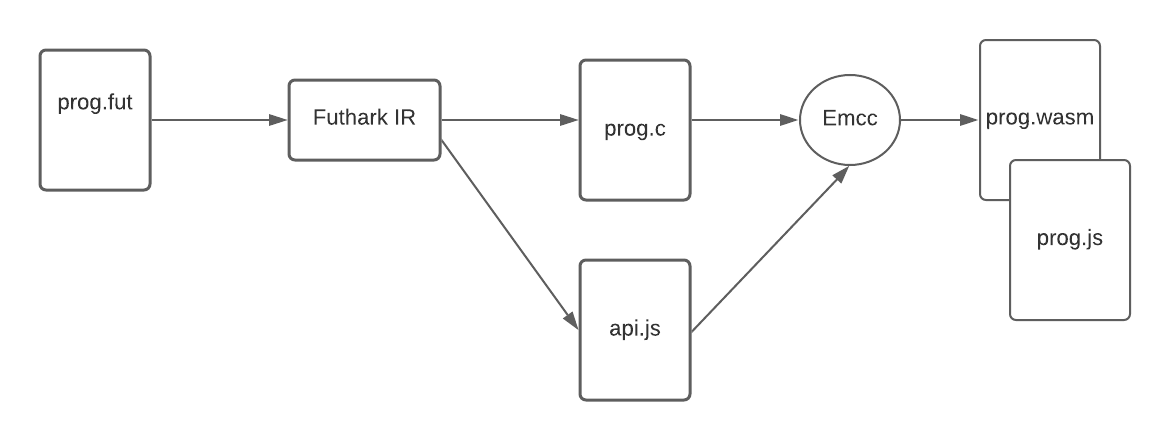
\includegraphics[width=\textwidth]{figures/compiler_pipeline.png}}
\caption{Sequential WebAssembly backend compiler pipeline}
\label{fig:wasm}
\end{figure}

The source program is turned into Futhark's intermediate representation, and then into C source code. Our JavaScript API classes that the WebAssembly backend generates only depend on the function names, argument types, and return types, which can be taken from the intermediate representation. At this stage both the C source code and the API are joined together with the EMCC command, generating glue code with the attached API classes, and a WebAssembly module. 

\subsection{Emscripten Compiler Flags}
The Emscripten compiler provides a large number of flags that effect the usage and the performance of the generated WebAssembly code. The backend implementation uses only a few flags. The WebAssembly backend implementation includes a facility for the user to specify further compiler flags to pass emcc, via the EMCFLAGS environment variable. This way the users of the WebAssembly backend can add the flags that are best suited for their applications. As discussed previously in order for 64-bit integers to be handled correctly, the backend needs to use the \texttt{WASM\_BIGINT} flag. The other flag that it defaults to is the O3 optimization level. Though this obfuscates the resulting code, it comes with sizeable performance improvements over the other optimization levels. Most browsers will have means to automatically pretty print the obfuscated code.

The most important flag for users of the WebAssembly backend to consider is the \texttt{INITIAL\_MEMORY} flag. The memory flag in Emscripten defaults to 16 megabytes, but with performance heavy computation it is likely that this limit will be exceeded. In these cases the user should manually set the memory based on their needs. It is recommended to use less than 2 gigabytes as only recently have virtual machines started to allow more than 2 gigabytes of heap space. This means that using more memory than 2 gigabytes will likely not be portable across browsers and with different WebAssembly engines. 

Listing \ref{lst:fu-wasm-compile} shows an example of calling the backend with an additional compiler flag to set the memory limit higher. The additional compiler flags to Emscripten are passed through the environment variable EMCFLAGS. In this case the memory is increased to 64 megabytes.

\begin{listing}
\begin{minted}{bash}
EMCFLAGS="-s INITIAL_MEMORY=$((16777216 * 4))" futhark wasm --lib prog.fut
\end{minted}
\caption{Example futhark wasm compile command}
\label{lst:fu-wasm-compile}
\end{listing}

\section{Application}
\label{sec:mandelbrot}

With the WebAssembly backend implemented as described above, it can now be seen in action. One of the applications for high performance computing in the browser is graphics. Figure \ref{fig:mandelbrot} illustrates a Futhark program running in the browser for visualizing the Mandelbrot set. 

The full implementation of \textit{mandelbrot.fut}
comes from ({\color{red} TODO})
and can be found in the appendix {\color{red} TODO}. Taking a look at the function signature:
\begin{minted}{Haskell}
let main (screenX: i64) (screenY: i64)
         (depth: i32) (xmin: f32)
         (ymin: f32) (xmax: f32)
         (ymax: f32): [screenY][screenX]i32 =
\end{minted}

We note that the entry point function takes 7 input arguments. The first two arguments \texttt{screenX} and \texttt{screenY} specify the dimensions of the output. 

We firstly compile the \textit{mandelbrot.fut} file as a library:
\begin{minted}{bash}
futhark wasm --lib mandelbrot.fut
\end{minted}
This generates the files \textit{mandelbrot.js} and \textit{mandelbrot.wasm}. At this stage we can write a HTML file to call the JavaScript API.

Listing \ref{lst:mandelbrot-html} is a web page that takes 7 inputs from the user, one for each of the arguments in the \textit{mandelbrot.fut} entry point function. The user can then click a button, which will then run the Mandelbrot computation and visualization by calling the Futhark function.

\begin{listing}[t!] 
        \inputminted[fontsize=\small,baselinestretch=0.5,linenos]{HTML}{code/examples/HTML/mandelbrot.js}
        \caption{HTML file for calling \textit{mandelbrot.js}}
        \label{lst:mandelbrot-html}    
\end{listing}


In order to run the code in the browser, we need to launch a web server. This can be done from Python with
\begin{verbatim}
python -m http.server
\end{verbatim}
After running the server, we can go the web page in any modern browser. Put in inputs and then press the button. Once the mandelbrot computation is complete the result will render in the page.


Figure \ref{fig:mandelbrot} shows the visualization once the function is done executing. The example illustrates how Futhark code can be compiled into a WebAssembly module that can be called in the browser. The WebAssembly module offload the computationally heavy workload from the less efficient JavaScript execution engine. The only Futhark specific code in listing \ref{lst:mandelbrot-html} are lines 27-30:
\begin{minted}{javascript}
var instance = await createFutharkModule();
var fc = new instance.FutharkContext();
var result = fc.main(screenX, screenY, depth, xmin, ymin, xmax, ymax);
var vals = result.toTypedArray();
\end{minted}
The first line loads the WebAssembly module. The second line instantiates the context. The third line runs the entry point function. And finally the fourth line converts the result FutharkArray to a standard JavaScript typed array. Observe that the user of this library doesn't need to be aware that there is any WebAssembly under the covers. 

\begin{figure}[h!]
    \centering
    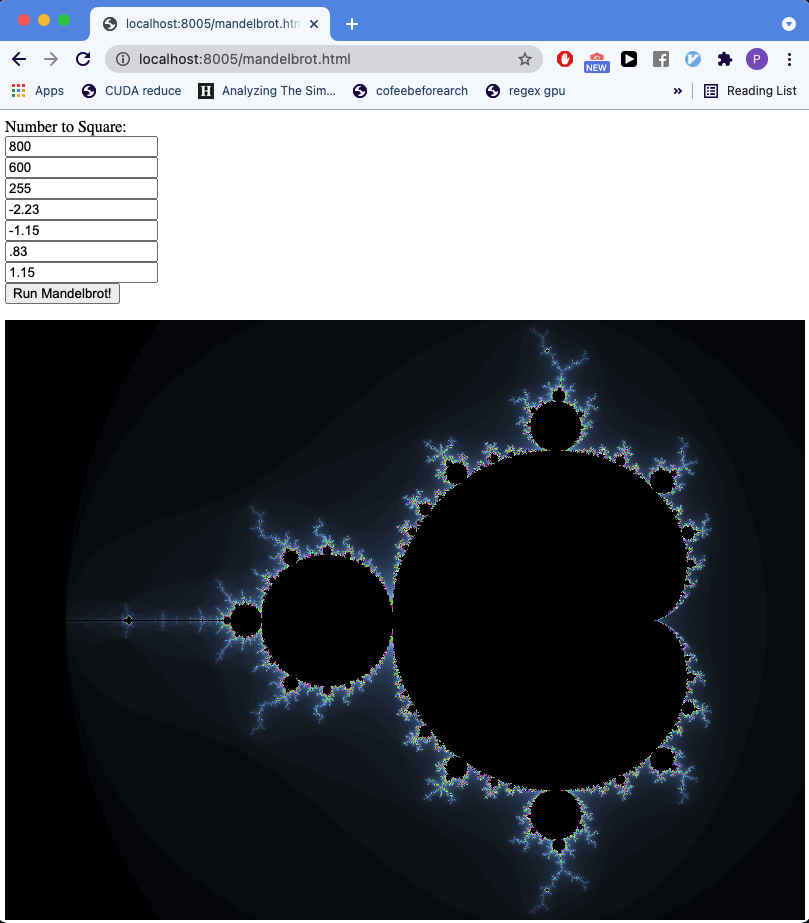
\includegraphics[scale=0.3]{figures/mandelbrot.png}
    \caption{Caption}
    \label{fig:mandelbrot}
\end{figure}




\section{Benchmarking}

The WebAssembly backend is benchmarked against the C backend to see how competitive the execution speed is. The WebAssembly backend is both benchmarked running in the browser with Chrome as well as running with Node. 
\begin{itemize}
    \item Chrome: benchmarking WebAssembly in Chrome gives details on how WebAssembly performs in the browser, which is likely where the backend will be deployed in practice.
    \item Node: benchmarking with Node gives details into how the WebAssembly preforms when run as a backend language. This is interesting as it gives details into the WebAssembly's performance for use cases outside of the browser.
\end{itemize}



The Futhark programs that are benchmarked come from the Futhark benchmark suite, which are used for standardized benchmarks to test the performance of all Futhark backends against industry standards. What is interesting to look at is how the WebAssembly performs relative to the C backend it is built on top of.
\begin{table}[h!]
    \noindent\makebox[\textwidth]{%
    \begin{tabular}{|l|l|l|l|l|l|}
    \hline
    Suite      & Dataset                     & Size & C        & WebAssembly     & Chrome \\ \hline
    \multirow{3}{*}{Accelerate} & \multirow{3}{*}{Tunnel} & 1000 & 735 ms  & 1,219 ms  & 1217  \\ \cline{3-6} 
               &                             & 2000 & 2,942 ms & 4,889 ms & 4,827 ms    \\ \cline{3-6} 
               &                             & 4000 & 11,762 ms & 19,693 ms & 19,302 ms   \\ \hline
    \end{tabular}%
    }
    \caption{Caption}
    \label{tab:my_label}
\end{table}

The Tunnel Benchmark shows that the WebAssembly backend takes approximately 65\% performance penalty for running the benchmarks with WebAssembly relative to the sequential C backend. This performance penalty is consistent as the dataset increases, which means that it is not a constant overhead of launching or instantiating WebAssembly. WebAssembly when run in Chrome and in Node have nearly identical performance, with the difference never exceeding 2 percentage points.

\begin{table}[h!]
    \noindent\makebox[\textwidth]{%
    \begin{tabular}{|l|l|l|l|l|l|}
    \hline
    Suite      & Dataset                     & Size & C        & WebAssembly     & Chrome \\ \hline
    \multirow{3}{*}{Accelerate} & \multirow{3}{*}{Mandelbrot} & 1000 & 131 ms   & 149 ms  & 155 ms  \\ \cline{3-6} 
               &                             & 2000 & 530 ms  & 602 ms  & 601 ms    \\ \cline{3-6} 
               &                             & 4000 & 2,117 ms & 2,403 ms & 2446 ms   \\ \hline
    \end{tabular}%
    }
    \caption{Caption}
    \label{tab:my_label}
\end{table}

For the mandelbrot benchmarks the WebAssembly backend has more competitive execution speeds. The WebAssembly backend is consistently 13-14\% slower across all the sizes. Similarly to the tunnel backend the relative performance difference of the C backend and the WebAssembly does not change with respect to the dataset sizes.


{\color{red} TODO} add more benchmarks

{\color{red} TODO} add more discussion

{\color{red} TODO} add conclusion
\chapter{Parallel Execution in the Browser}


Browsers have facilities for parallel programming. Javascript supports two different paradigms with web workers. Message passing enables parallel programming without shared memory. SharedArrayBuffer and atomics enable shared memory multithreading with thread synchronization. There is a threaded WebAssembly proposal that adds atomic operations to the language, and adds support for SharedArrayBuffers while relying on JavaScript's web workers to create and join threads. This chapter introduces all these concepts and illustrates them with examples.

%JavaScript is single threaded. Meaning it consists of a single call stack and a single memory heap. This is slightly counter intuitive as idiomatic JavaScript often contains many asynchronous function calls. Asynchronous function calls are achieved by placing promises/callbacks into an event queue, which runs after the main thread has finished processing. This way they avoid blocking synchronous JavaScript code from running. 

%There are three primitives used for doing multithreaded programming in the browser: Web Workers, Shared Memory, and Atomics. These features will be introduced in this section along with examples illustrating how they are used in practice. 


\section{Web Workers}
Parallelism with JavaScript in browsers is achieved through web workers. Web workers are extra threads of execution beyond the main thread. The threads interact via message passing. Typically messages are passed through the postMessage and onmessage. postMessage is used to send a message between threads and onmessage works as an event handler to receive messages from threads. 


Web workers are relatively heavyweight, and should not be created in large numbers. They are expected to be long lived and have both high start and high per instance memory cost. 
{\color{red} TODO} show why/where this information comes from (FOLLOW UP FROM ABOVE)

The following example computes the Riemann integral of sine over an interval from 0. The interval is broken up into subintervals which are computed by separate workers.

\begin{listing}[H] 
        \inputminted[fontsize=\small,baselinestretch=0.5,linenos]{javascript}{code/worker/integrate.js}
        \caption{Main file that calls workers which handle the computation of Riemann integral} 
        
        \label{lst:integrate-js}    
\end{listing} 

The example code in Listing \ref{lst:integrate-js} spawns 4 worker threads in lines 5-7. It sends each thread a message with their respective index in lines 18-20. It asynchronously waits for messages from each of the worker threads with their partial result and prints the final result when all the threads have sent a message in lines 10-16.
\begin{listing}[H] 
        \inputminted[fontsize=\small,baselinestretch=0.5,linenos]{javascript}{code/worker/worker.js}
        \caption{Worker thread logic for computing Riemann integral} 
        \label{lst:worker-js}    
\end{listing}    

The code in Listing \ref{lst:worker-js} contains the implementation of the worker threads. Once the thread receives a message from the main thread with their index, they compute the partial Riemann integral over their respective quartile of the interval adding the value of sine(x) as many times as specified by granularity. Figure \ref{png:integrate} shows the execution time of the code against a different number of web workers.



\begin{figure}[H]
\centerline{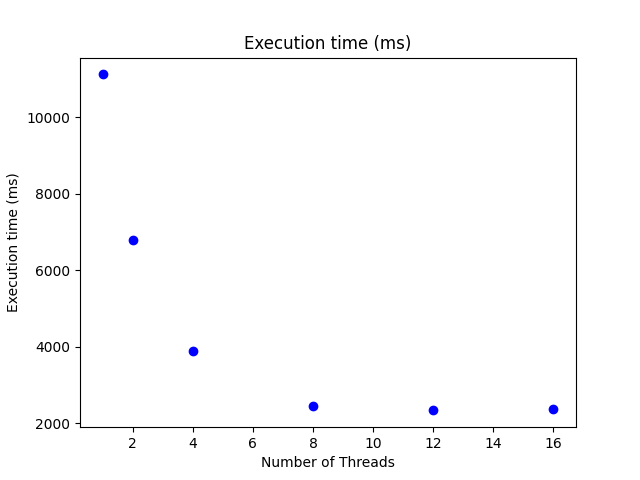
\includegraphics[width=\textwidth]{figures/integrate_exe_times.png}}
\caption{Execution time of Riemann integration for different thread counts. Run on a Macbook Pro with 2,2 GHz 6-Core Intel Core i7}
\label{png:integrate}
\end{figure}

The code execution time in \ref{png:integrate} is for the Reimann integral computed with one billion sample values. For one worker thread the execution time was 11.11 seconds. For two threads the execution time was 6.8 seconds, which is nearly double as fast. However as the number of threads increases the increase in execution speed tapers off. Going from 8 to 12 cores only yields a marginal increase in execution speed going from 2.45 second to 2.39. Once more than twelve worker threads are exceeded, there is no longer a marginal increase in speedup. This can be attributed to the physical limitation of threads on the hardware the code was executed on. The number of logical cores on the computer that executed this code was 12, meaning that any additional web worker launched after the initial 12 must wait on the thread pool for another to finish before it can be activated. In which case the overhead of launching it is only detrimental to the complete execution time of the program


\section{Shared Memory and Atomics}

Web workers with message passing have some similarities in how parallelism is executed with the Erlang programming language. Both of which use message passing to coordinate parallel execution. However many other programming languages and libraries also support and utilize shared memory. An example of this is C/C++ and POSIX threads. Shared memory maps closely to modern multicore hardware, and is faster for certain workloads ({\color{red} TODO} GIVE EXAMPLE). However it comes at the cost of a new set of bugs in the shape of data races, which is why languages such as Erlang and Futhark itself abstracts the construct away from the programmer.
\begin{listing}[t!]    
        \inputminted[fontsize=\small,baselinestretch=0.5,linenos]{javascript}{code/shared/main.js}
        \caption{Main file that calls workers which compute prefix sum using shared memory and atomics in parallel}    
        \label{lst:main-js}    
\end{listing}    
JavaScript also offers shared memory through SharedArrayBuffers. A SharedArrayBuffer points to a piece of linear memory. The SharedArrayBuffer can be passed to multiple web workers who can access the memory in parallel. 

In principle safe access to shared memory can be coordinated with message passing, but it's far more efficient for fine grained synchronization to use atomic operations, which again map efficiently to the underlying hardware. Atomic operations make sure that predictable values are written and read, that operations are finished before the next operation starts and that operations are not interrupted \cite{js-atomics}. The Atomics package in JavaScript contains functions for performing atomic operations on SharedArrayBuffers. The Atomics package also includes wait and notify functions, like linux futex, wait, and wake.
%\captionof{listing}{Example of a worker working}
\begin{listing}[b!]    
\inputminted[fontsize=\small,baselinestretch=0.5,linenos]{javascript}{code/shared/prefix_sum.js}
        \caption{Worker file for computing the prefix sum using shared memory and atomics.}    
        \label{lst:prefixsum-js}    
\end{listing}    

To illustrate shared memory and atomics the following example is an implementation of prefix sum. It is a fundamental parallel algorithm which is used as a building block for many other parallel algorithms. The example implements the shared memory 2 pass algorithm from ({\color{red} TODO}). 

The code in Listing \ref{lst:main-js} spawns 9 worker threads. It sends a message to each of the threads with parameters, some of which are shared array buffers. This allows each of the threads to have access to shared memory. When each thread has sent a message to indicate completion, the final result of prefix sum is logged to the console.



The code in Listing \ref{lst:prefixsum-js} handles the actual execution of prefix sum. In the first pass of the algorithm, each thread calculates the prefix sum of their partition in the array, by calling the function \texttt{prefix\_sum\_partition}. Each thread signals that they are done with their work in the first pass by using the Atomics add, and notify functions. The first thread detects signal has accumulated a response of \texttt{num\_workers - 1}, by using the Atomics function wait. At this point the the first thread calculates the cumulative sums of partitions. At this stage it notifies the other other threads using the Atomics store and notify. At this stage all threads calculate the final \texttt{prefix\_sum}, using the precomputed values. On completion each thread sends a message back to the the main file using the postMessage to indicate they are done. 


%{\color{red} TODO}: Show speed up over one worker vs 9 workers

%{\color{red} TODO} update code to be cleaner and easier to explain

\section{Threaded WebAssembly}
There is a proposal to extend the WebAssembly specification with support for threads, namely by leveraging web workers, shared memory, and atomics. Chrome and Firefox and Node.js all have experimental support for threaded WebAssembly. Emscripten supports compilation of C/C++ with pthreads to threaded WebAssembly.

Threaded WebAssembly uses web workers to create and join threads. It doesn't natively invoke web workers but instead handles this by calling out to JavaScript. Shared memory is accomplished by integrating SharedArrayBuffer with WebAssembly's paged memory model. WebAssembly is extended with atomic operation instructions. Putting it concisely the additions of supporting shared array buffers in WebAssembly and adding atomic operations in WebAssembly was all that was needed to facilitate threaded WebAssembly.

A key observation is that WebAssembly does not natively allow for spawning of threads. This is actually taken care of by the runtime or compiler. Specifically for Emscripten, compiling C code written with pthreads will generate three files. It will generate a WebAssembly file, and and two Javascript files. One for the main glue code and other for worker glue code. The glue code takes care of loading the WebAssembly module, populating the memory with the required values, and integrating with the host system as the C code would expect. The C function pthread\_create is translated to Javascript and not WebAssembly. It launches a Javascript Worker, passing it a shared array buffer and the wasm module that it should run. The WebAssembly simply needs the shared array buffer and atomics to synchronize.  

\begin{figure}[htb]
\centerline{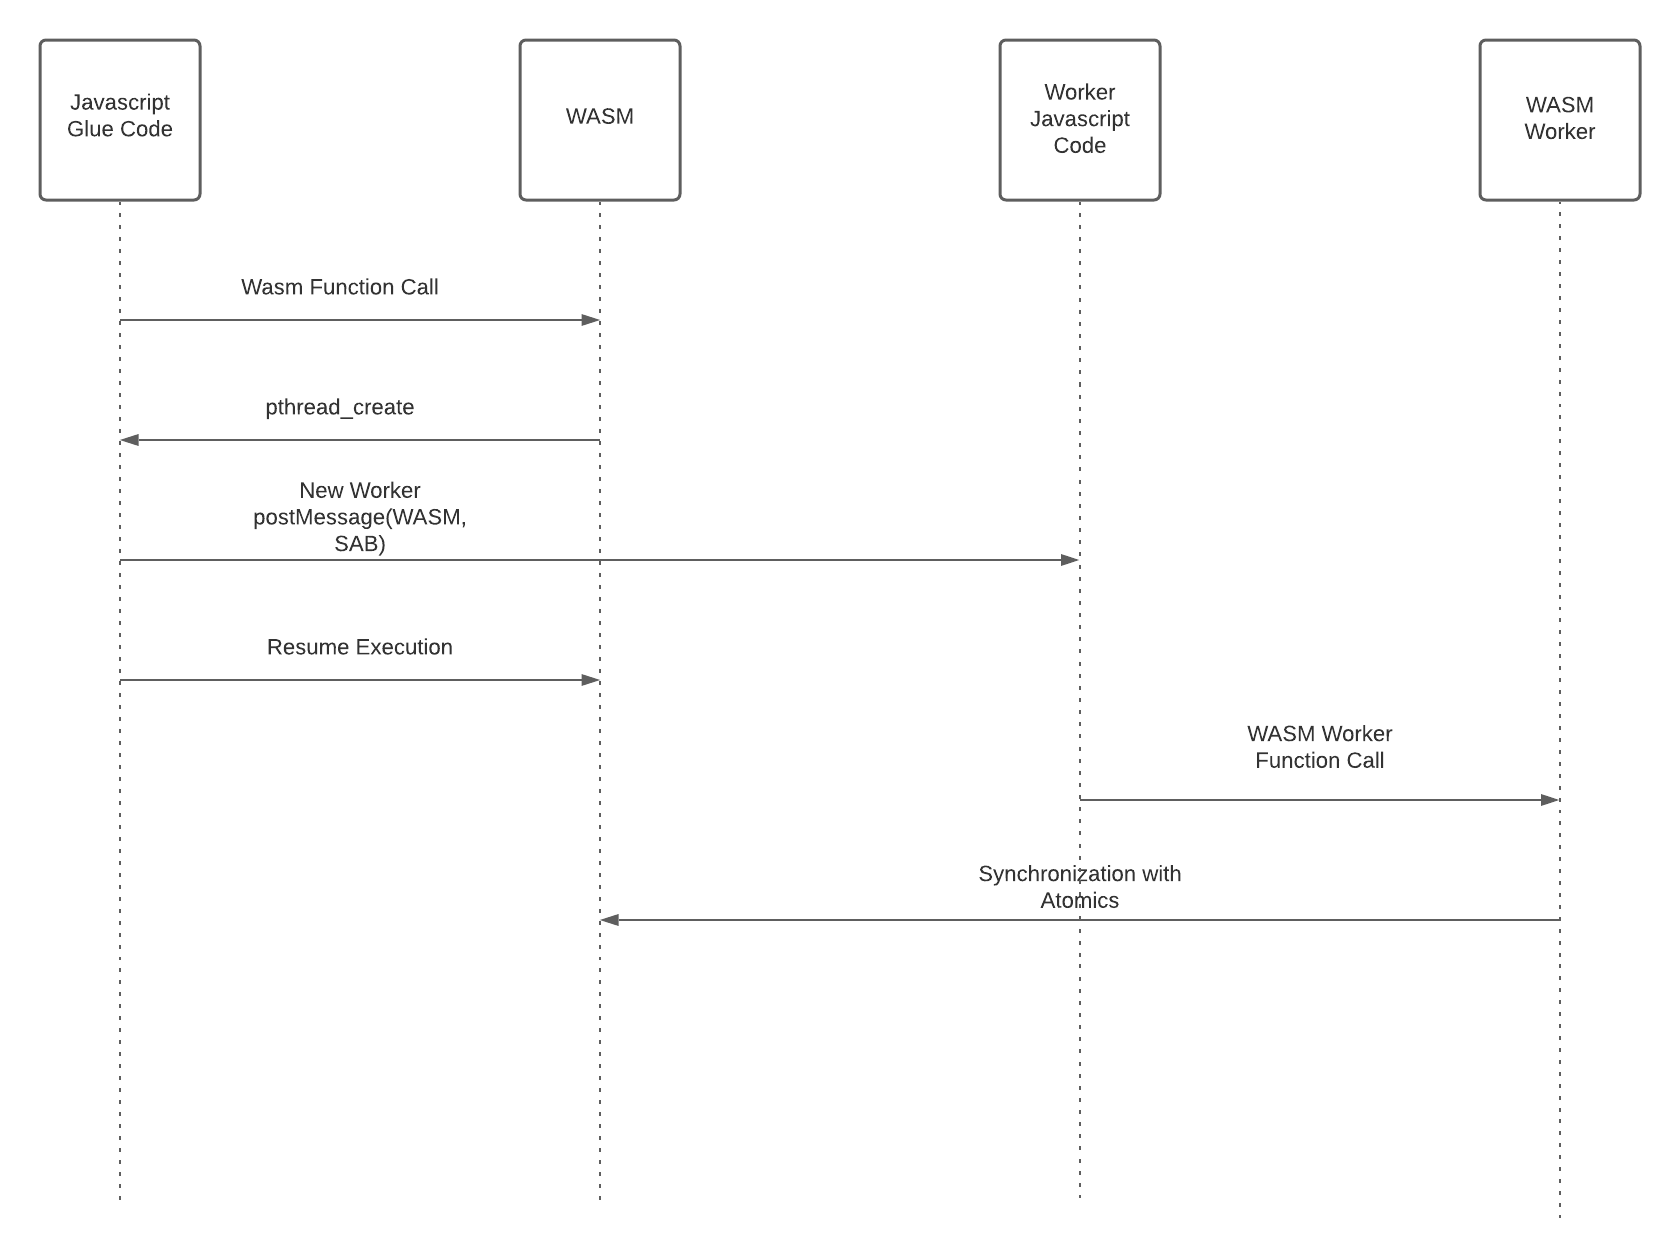
\includegraphics[width=\textwidth]{figures/UML_threaded_wasm.png}}
\caption{UML diagram showing flow of execution of threaded programs in WebAssembly}
\label{uml}
\end{figure}

%{\color{red} TODO} make updates to UML as specified on piece of paper.

The UML diagram in figure \ref{uml} demonstrates the execution flow of a parallel function written with pthreads in C, compiled by Emscripten, and run in Javascript and WebAssembly. The javascript glue code calls the parallel WebAssembly function, which then calls an external Javascript function that is used to emulate the functionality of \texttt{pthread\_create}. This function launches a new worker, sending it a message with the WebAssembly module, and a shared array buffer, and resumes execution. This JavaScript worker code then  instantiates the WebAssembly module, calling the designated WebAssembly module function. And then with these multiple WebAssembly modules running in parallel, they use atomic instructions native to WebAssembly to facilitate synchronization, as specified in the program.

%{\color{red} TODO}: Pthreads + memory growth talk about this

%{\color{red} TODO}: Talk about specifying number of web workers up front with Emscripten

%{\color{red} TODO} Explain why threaded WebAssembly has no drawbacks becuase it uses the same facilites as javascript for parralel programming while having the speed up of WebAssembly over JS. (Possibly look at over head of launching/loading WebAssembly in a JS worker file).

\newpage
\chapter{WebAssembly Multicore Backend}

This chapter details the extensions that are added to the Futhark compiler to support a multicore WebAssembly backend. It also benchmarks the generated WebAssembly-multicore code against the sequential WebAssembly backend. It also compares the multicore C backend against the WebAssembly-multicore backend running in the browser.

Fortunately only small adaptions had to be made to the WebAssembly backend developed earlier, to get it running with Multicore. The Futhark compiler has a backend that generates both Sequential C code as well as a backend that generates multicore C code using POSIX threads. As discussed Emscripten can translate multicore C code that uses POSIX threads to multicore WebAssembly that can run in parallel in the browser. The JavaScript API developed in chapter 4 stays most unchanged, with only one small modification for the WebAssembly-multicore backend. 

Though this thesis adds 2 backends to the 6 backends already present in the Futhark compiler (4 C backends, and 2 Python backends), the added complexity is relatively modest because of the high degree of reuse of code between the two WebAssembly backends. 


\section{Implementation Structure}

Below we discuss how to add a new futhark backend that can be invoked from the command line with \texttt{futhark wasm-multicore}. It is structured very similarly to the plain WebAssembly backend described chapter 4. Instead of calling Emscripten on the Sequential C, we apply it to Futhark's multicore C backend. We utilize the JavaScript and WebAssembly runtime code written in chapter 4, for the backend and add the necessary Emscripten compiler flags required to enable Multicore WebAssembly. Figure \ref{fig:wasm-mc} illustrates the structure of the WebAssembly multicore implementation.

\begin{figure}[htbp]
\centerline{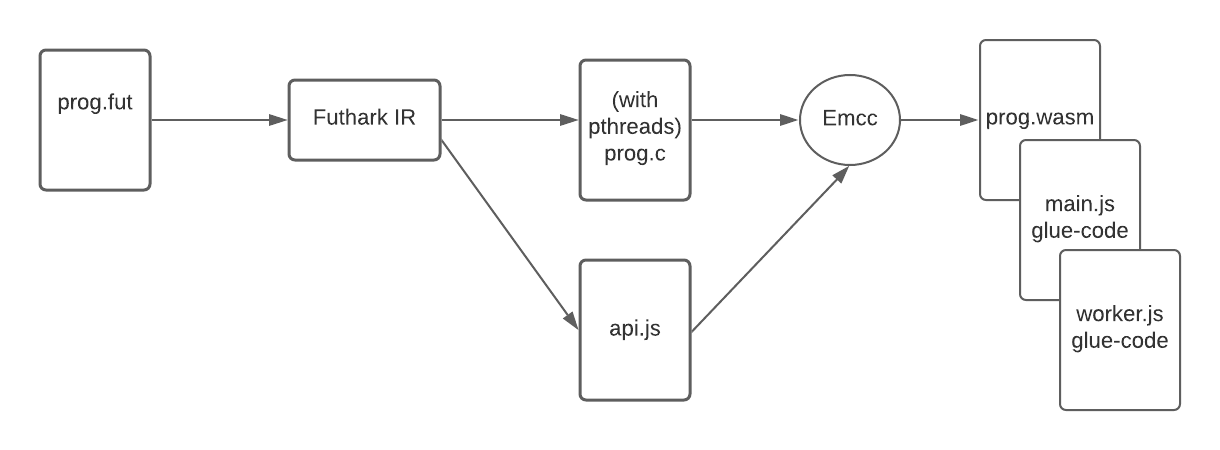
\includegraphics[width=\textwidth]{figures/WASM_MC_compiler.png}}
    \caption{WebAssembly-multicore compilation}
\label{fig:wasm-mc}
\end{figure}
One of the key differences that can be seen in the figure \ref{fig:wasm-mc} is that the wasm-multicore backend produces 2 JavaScript files and 1 WebAssembly file as opposed to the Sequential Wasm backend which generates 1 JavaScript file and 1 WebAssembly file. The second JavaScript file is the web worker glue code.

\section{Implementation Details}
Here we discuss the series of steps that were needed complete the implementation.
\subsection{Plumbing}

We simply combine the multicore C compiler with the JavaScript code generation discussed in chapter 4, by calling the respective functions that contain the meat of the logic, which have already been developed. The last thing of note is that the flag \texttt{-pthread} is passed to \texttt{runEMCC}. This flag lets Emcc know that our C code contains pthreads, and thereby compiles it correctly. %OBS


\subsection{Multicore C code changes}
The pthread C code generated by the multicore C backend used platform specific implementations in the generated function \texttt{getrusage\_thread} and \texttt{num\_processors}. For \texttt{getrusage\_thread} it was possible to reuse the linux implementation. For \texttt{num\_processors} it was necessary to add an additional implementation for the Emscripten platform. This was simply done by including \textit{emscripten/threading.h} and calling the function \texttt{emscripten\_num\_logical\_cores}. %OBS


\subsection{API Change}
The multicore C backend exports one important additional function for setting the number of threads the library will use:
\begin{verbatim}
void futhark_context_config_set_num_threads(
     struct futhark_context_config *cfg, int n);
\end{verbatim}
\texttt{futhark\_context\_config\_set\_num\_threads} does this by taking threads and configuration as argument and then number of threads that the library will use on the configuration. This information we would like to have when running our library. We adapt our API to pass an an optional argument to the FutharkContext constructor:
\begin{listing}[H]
    \inputminted[fontsize=\small,baselinestretch=0.5,linenos]{JavaScript}{code/compiler/api_examples/FutharkContext-opt.js}
    \caption{FutharkContext with optional argument}    
    \label{lst:fut-opt}    
\end{listing} 
 
 In the constructor in listing \ref{lst:fut-opt} we simply set the number threads to be the argument given in the FutharClass constructor. If no argument is given, it defaults to \texttt{emscripten\_num\_logical\_cores}. Surprisingly this was the only adaption we needed to make in the API described in chapter 4.
\subsection{Emscripten Invocation}

The generated multicore C code uses the POSIX function \texttt{pthread\_create}. Emscripten aims to follow the POSIX standard closely, but in some places has slightly different behaviour. This is the case for \texttt{pthread\_create}, which is a function that is used in the generated multicore C code. 

When pthread\_create() is called, if we need to create a new Web Worker, then that requires returning the main event loop. That is, you cannot call \texttt{pthread\_create} and then keep running code synchronously that expects the worker to start running - it will only run after you return to the event loop \cite{pthread-doc}. In order to work around the API differences, the compiler flag \texttt{PTHREAD\_POOL\_SIZE=<integer>} needs to be passed to the Emscripten compiler. This effectively creates the web workers before the main thread is called, in which case \texttt{create\_pthread} can just use an already spawned web worker. From testing, this parameter is best set to the number of \texttt{logical\_cores} of the underlying hardware. %OBS






\subsection{Running in browser with HTTP}

Running threaded WebAssembly in the browser is slightly more involved than running standard WebAssembly. This is because threaded WebAssembly uses SharedArrayBuffers. SharedArrayBuffers introduce a few security vulnerabilities. For this reason browsers require us to set to HTTP headers when we run our web server. We need to set the flags as follows:
\begin{itemize}
    \item Cross-Origin-Embedder-Policy (COEP) : require-corp
    \item Cross-Origin-Opener-Policy (COOP) : same-origin
\end{itemize}

The following listing \ref{lst:server} file can be used to run a web server with COEP and COOP headers set:

We can run this Python file, to run threaded WebAssembly programs locally.

\begin{listing}[H]    
        \inputminted[fontsize=\small,baselinestretch=0.5,linenos]{Python}{code/server.py}
        \caption{Python server implementation for setting COEP and COOP HTTP Headers}    
        \label{lst:server}    
\end{listing} 



\subsection{Applications}

In order to see the WebAssembly multicore code in action, we will use ray tracing as a motivating example. Ray tracing is a technique in graphics, which is used to simulate how rays of light bounce off objects. Ray tracing can be used to create realistic, high definition pictures. Its a common technique used in rendering and movies.

{\color{red} TODO}: Put raytrace.fut in append
{\color{red} TODO}: Reference raytrace.fut in appendix
{\color{red} TODO}: say where i got it from 
We are mainly concerned with the arguments and return type of the entry point function. The entry point for \textit{raytracer.fut} is defined as follows:
\begin{minted}{Haskell}
let main (nx: i64) (ny: i64) 
         (ns: i32) (nobj: i32) 
         : [ny][nx]argb.colour
\end{minted}
The function takes \textbf{nx} and \textbf{ny} specifying the number of pixels we want our ray tracer to cover. This \textbf{ns} specifies the number of samples we want per pixel. Lastly nobj specifies the number of reflections per ray. The return type is a grid of \texttt{u32} numbers. 


We can can compile the WebAssembly library with the following command

\begin{verbatim}
EMCFLAGS="-s INITIAL_MEMORY=2147418112 -s PTHREAD_POOL_SIZE=12" \ 
                         futhark wasm-multicore --lib raytracer.fut
\end{verbatim}

With this command we are giving WebAssembly access to approximately 2 gigabytes and setting the number of threads to be run simaltaniusly to 12. The result of this command will be three files: \textit{raytracer.js}, \textit{raytracer.worker.js}, and \textit{raytracer.wasm}. Listing \ref{lst:raytracer} shows an example HTML page that calls the compiled Futhark library.
\begin{listing}[t]    
        \inputminted[fontsize=\small,baselinestretch=0.5,linenos]{HTML}{code/examples/HTML/raytrace.js}
        \caption{HTML file for creating ray trace visualization}    
        \label{lst:raytracer}    
\end{listing} 

The web page has a button, which runs a function. This function loads the Futhark library, and instantiates FutharkContext. It then calls the Futhark entry point with the arguments 400, 400, 50, and 5 for \textbf{nx}, \textbf{ny}, \textbf{ns}, and \textbf{nobj} respectively. It proceeds to display the result on the page. With this HTML file, compiled Futhark library, and the Python server file from \ref{lst:server} we can run the code.

We simply run the Python file (it launches a web server with the appropriate configuration), and then go to \texttt{localhost:8000}. Figure \ref{fig:raytrace} shows the state of the web page after the button has been clicked and it has finished executing. 

\begin{figure}[htb]
    \centering
    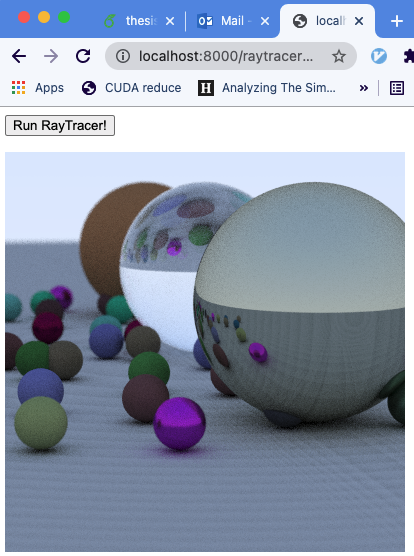
\includegraphics[scale=0.6]{figures/raytracer.png}
    \caption{Caption}
    \label{fig:raytrace}
\end{figure}

\section{Benchmark}

\begin{table}[h!]
    \noindent\makebox[\textwidth]{%
    \begin{tabular}{|l|l|l|l|l|l|}
    \hline
    Suite      & Dataset                     & Size & C        & WebAssembly     & Chrome \\ \hline
    \multirow{3}{*}{Accelerate} & \multirow{3}{*}{Mandelbrot} & 1000 & 14.7 ms   & 39 ms  & 27 ms  \\ \cline{3-6} 
               &                             & 2000 & 53 ms  & 103 ms  & 104 ms    \\ \cline{3-6} 
               &                             & 4000 & 211 ms & 412 ms & 532 ms   \\ \hline
    \end{tabular}%
    }
    \caption{Caption}
    \label{tab:my_label}
\end{table}


\begin{figure}
    \centering
    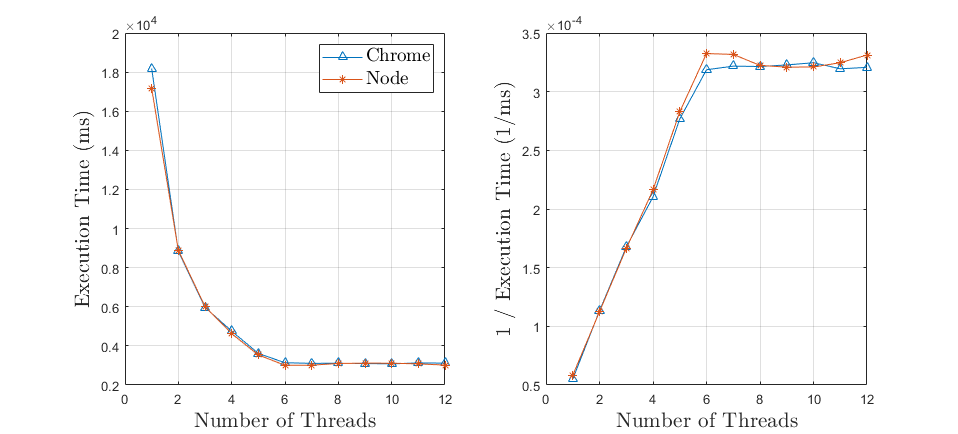
\includegraphics[width=\textwidth]{figures/execution_time.png}
    \caption{Caption}
    \label{fig:benchtime}
\end{figure}
\chapter{Conclusion}

This thesis has made several contributions toward extending high level and high performance parallel programming to modern consumer devices.
New WebAssembly and threaded WebAssembly backends were developed for the Futhark compiler to compile Futhark functions to WebAssembly modules that run efficiently in the browser. Furthermore, to call the WebAssembly modules from the browser, an efficient, convenient, and concise JavaScript API was developed and illustrated with examples. 
The backends and API were implemented in Haskell as additions to Futhark’s open source compiler and were benchmarked to prove their efficiency and the performance gains that can be obtained with multithreading on multicore computers.
The utility of compiling Futhark to WebAssembly was tested with Mandelbrot and ray tracing, two working visualization programs that generate and display images in the browser.
\newpage
\section{Attempt}

This thesis has presented the design and implementation of two new backends for Futhark targeting WebAssembly and threaded WebAssembly, enabling efficient execution of sequential and parallel in the browser. 

We began, in chapter 2, by surveying the technologies, present and emerging, for doing high performance and parallel programming in the browser. WebAssembly was identified as a promising technology due to its <{\color{red} TODO} more here> and the multithreading support in the experimental extension, threaded WebAssembly. The details of WebAssembly and Emscripten, in chapter 3, and threaded WebAssembly, in chapter 6, were presented.

We designed a JavaScript API in chapter 4, for calling the compiled Futhark libraries from the browser, taking inspiration from APIs for calling Futhark libraries in C and Python. The resulting API is concise and efficient.

A new WebAssembly backend was developed for Futhark, implementing the API described in chapter 4. The backend was implemented taking the C code emitted by the sequential C backend and passing it to the Emscripten compiler, which generates a WebAssembly Module which can then be run in the browser. The new WebAssembly backend is demonstrated by computing and visualizing a mandelbrot set in the browser.

This new WebAssembly backend was 
%\item Survey technologies for high performance and parallel programming in the browser.

%\item Design an API for interoperation between Futhark and browser applications.

%\item Implement Futhark backends that generate libraries that run efficiently and in parallel in browsers.

%\item Evaluate the performance of these backends. 

%Chapter 2 explained the background of programming languages in the browser and parallel 

{\color{red} TODO}: explained background and related work

{\color{red} TODO}: explained WebAssembly and Emscripten, demonstrated with examples

{\color{red} TODO}: described JS API design and implementation, demonstrated with examples

{\color{red} TODO}: described WebAssembly Haskell implementation

{\color{red} TODO}: test suite

{\color{red} TODO}: benchmarks

{\color{red} TODO}: explained parallel execution in browsers, both in JS and with threaded WebAssembly, demonstrated with examples

{\color{red} TODO}: described threaded WebAssembly Haskell implementation, how to run it in the browser, with benchmarks

{\color{red} TODO}: reiterate that the goals of the thesis were met


{\color{red} TODO} fix incomplete bibtex



\appendix
\chapter{Source Code}

\section{GenericWASM.hs}
\begin{longlisting}
\inputminted[fontsize=\small,baselinestretch=0.5,linenos,breaklines]{Haskell}{code/compiler/codegen/GenericWASM.hs}
        \caption{Haskell source code for JavaScript wrapper code generation}    
        \label{lst:generic_wasm}    
\end{longlisting}  

\section{mandelbrot.fut}
\begin{longlisting}
\inputminted[fontsize=\small,baselinestretch=0.5,linenos,breaklines]{ocaml}{code/examples/futhark/mandelbrot.fut}
        \caption{mandelbrot.fut source code}    
        \label{lst:mandelbrot-src}    
\end{longlisting}  

\section{raytracer.fut}
\begin{longlisting}
\inputminted[fontsize=\small,baselinestretch=0.5,linenos,breaklines]{ocaml}{code/examples/futhark/raytracer.fut}
        \caption{raytracer.fut source code, originally taken from \url{https://github.com/athas/raytracinginoneweekendinfuthark}}    
        \label{lst:raytracing-src}    
\end{longlisting}  



\printbibliography[heading=bibintoc]

\afterpage{\blankpage}
\end{document}
